% Chapter 2

\chapter{Results} % Main chapter title

\label{Chapter4} % For referencing the chapter elsewhere, use \ref{Chapter4} 

% =========================================================== %
%          Subsection: Random Foraging                        %
% =========================================================== %
% \section{Random Foraging}
% \label{chap4:sec:1:RF_1p}
% \begin{itemize}
%     \item Significant decrease in information content in place cells
%     \item Differences in place fields properties (?)
% \end{itemize}

% =========================================================== %
%          Subsection: Open Field                             %
% =========================================================== %
% \section{Open Field}
% \label{chap4:sec:2:OF_1p}
% \begin{itemize}
%     \item Significant decrease in information content in place cells
%     \item Differences in place fields properties (?)
% \end{itemize}

% =========================================================== %
%          Subsection: Linear Track                           %
% =========================================================== %
\section{Pharmacogenetic manipulation of astrocytic calcium activity in vivo}
\label{chap4:sec:3:astro_dreadd}
In this thesis, we developed an analysis pipeline to investigate the effects of the manipulation of astrocytic calcium signals on neuronal spatial information encoding. 
Astrocytic calcium signals were manipulated by pharmacogenetic intervention using designer receptors exclusively activated by designer drugs (DREADD) technology [\cite{roth2016dreadds}; \cite{armbruster2005creation}; \cite{armbruster2007evolving}]. 
DREADDs (Figure \ref{fig:chap4:intro_dreadd_molecular}) perform signal transduction upon binding with their specific designer drugs. 
The DREADD receptor agonist is clozapine-n-oxyde (CNO), which is an endogenous product of the oxidative metabolism of clozapine.
\begin{figure}[h]
    \centering
    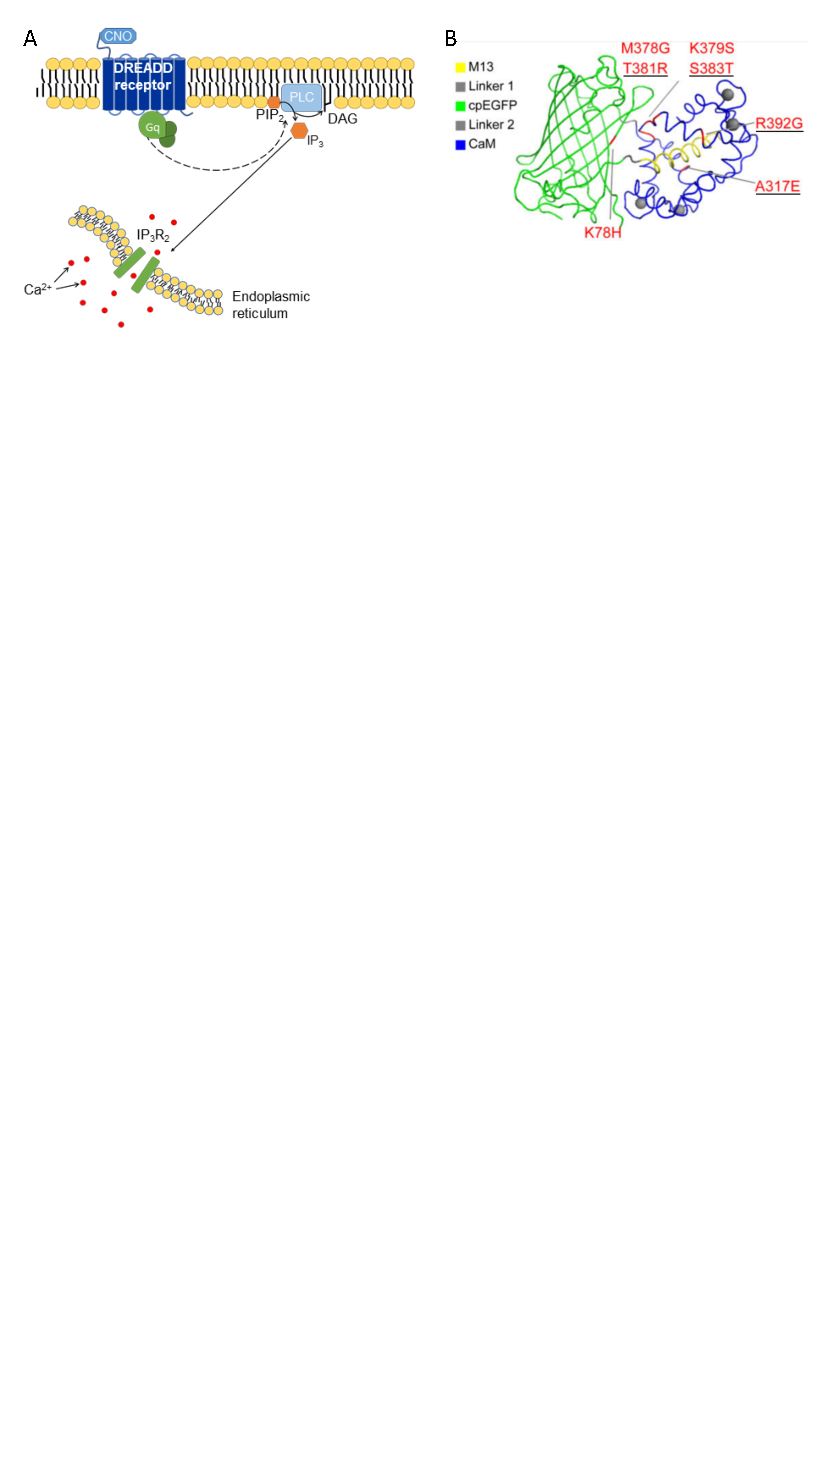
\includegraphics[trim={0 540 0 0},clip,width=\textwidth]{Figures/Chapter4/intro_dreadd_molecular.pdf}
    \caption[Tools used to manipulate and visualize astrocytic calcium signaling]{\textbf{Tools used to manipulate and visualize astrocytic calcium signaling.} 
    A) DREADDs (designer receptors exclusively activated by designer drugs) are engineered GPCRs that can be activated by inert chemicals and not by endogenous ligands. 
    We used the hM3Dq-receptor moiety, which is designed to bind CNO, mediating the activation of the Gq GPCR pathway. 
    In astrocytes, this pathway activates the signaling cascade of inositol 1,4,5-trisphosphate receptor (IP3R), mediating $Ca^{2+}$ release from the endoplasmic reticulum (ER). 
    B) GCaMP6f is a fast variant of the GCAMP family of genetically encoded calcium indicators (adapted from \cite{chen2013}) (Kd $375\ nM$). 
    To investigate calcium dynamics either in astrocytes or neurons, we relied on cell-specific promoters and optimized rAAV tropism (see methods \ref{chap3:sec:1:subsec2:AAV_injection}).}
    \label{fig:chap4:intro_dreadd_molecular}
\end{figure}
Upon binding, DREADDs rely on intracellular PKC machinery to activate G-protein coupled receptor (GPCR) signaling pathways (Figure \ref{fig:chap4:intro_dreadd_molecular}). 
DREADDs were generated in two classes to selectively manipulate either the Gq or Gi intracellular pathway. 
We selected the hM3Dq version of the DREADD receptor because it allowed spceific action on the Gq pathway. 
This manipulation was previously shown to promote calcium elevations in astrocytes [\cite{mu2019}; \cite{adamsky2018astrocytic}]. 
Throughout this thesis, hM3Dq activation was mediated via intraperitoneal injection of CNO (see methods \ref{chap3:sec:1:subsec2:AAV_injection}). 
In both astrocytes and neurons (see methods \ref{chap3:sec:1:subsec2:AAV_injection}) calcium activity was monitored using the fast genetically encoded calcium indicator GCaMP6f (Figure \ref{fig:chap4:intro_dreadd_molecular}B). 
\begin{figure}[h]
    \centering
    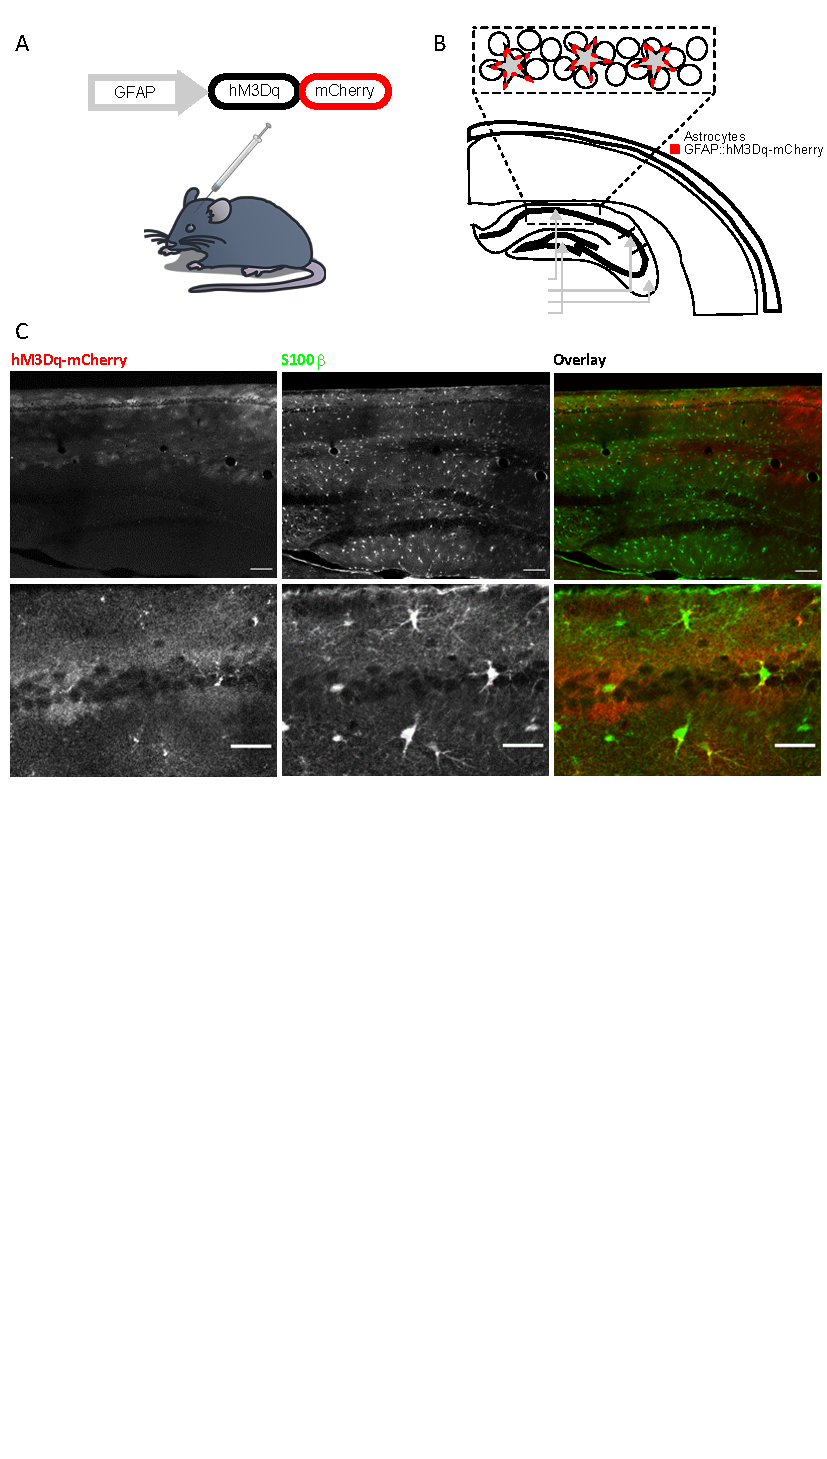
\includegraphics[trim={0 320 0 0},clip,width=\textwidth]{Figures/Chapter4/mcherry_dq_expression.pdf}
    \caption[Viral strategy to perform temporally restricted pharmacogenetic perturbation of astrocytic calcium signaling.]{\textbf{Viral strategy to perform temporally restricted pharmacogenetic perturbation of astrocytic calcium signaling.} 
    A) Adult mice were injected with serotype 5 rAAV encoding for the fusion construct hM3Dq-mCherry under the control of the astrocyte-specific promoter GFAP. 
    Injection was performed using stereotaxic coordinates to target the right hippocampus. 
    B) Schematic of virally transduced astrocytes in hippocampal CA1 area. 
    C) Confocal micrographs of CA1 area of mice expressing hM3Dq-mCherry construct. Astroglia was immunolabeled with the astrocyte-specific marker $S100\beta$. 
    Top: low magnification micrographs highlighting infection diffusion (scale $= 100\ \mu m$). 
    Bottom: high magnification micrographs show that the expression of hM3Dq-mCherry construct is restricted to astrocytic cell membrane (scale $= 30\ \mu m$).}
    \label{fig:chap4:mcherry_dq_expression}
\end{figure}

We used recombinant adeno-associated viral particles (rAAV) to deliver a DREADD-hM3Dq-mCherry fusion construct (hM3Dq-mCherry) into astrocytes.
The construct was under the control of the astrocyte-specific promoter GFAP (Figure \ref{fig:chap4:mcherry_dq_expression}A), and rAAV particles were pseudotyped with serotype-5 capsid proteins to improve astrocytic tropism.
\begin{figure}[h!]
    \centering
    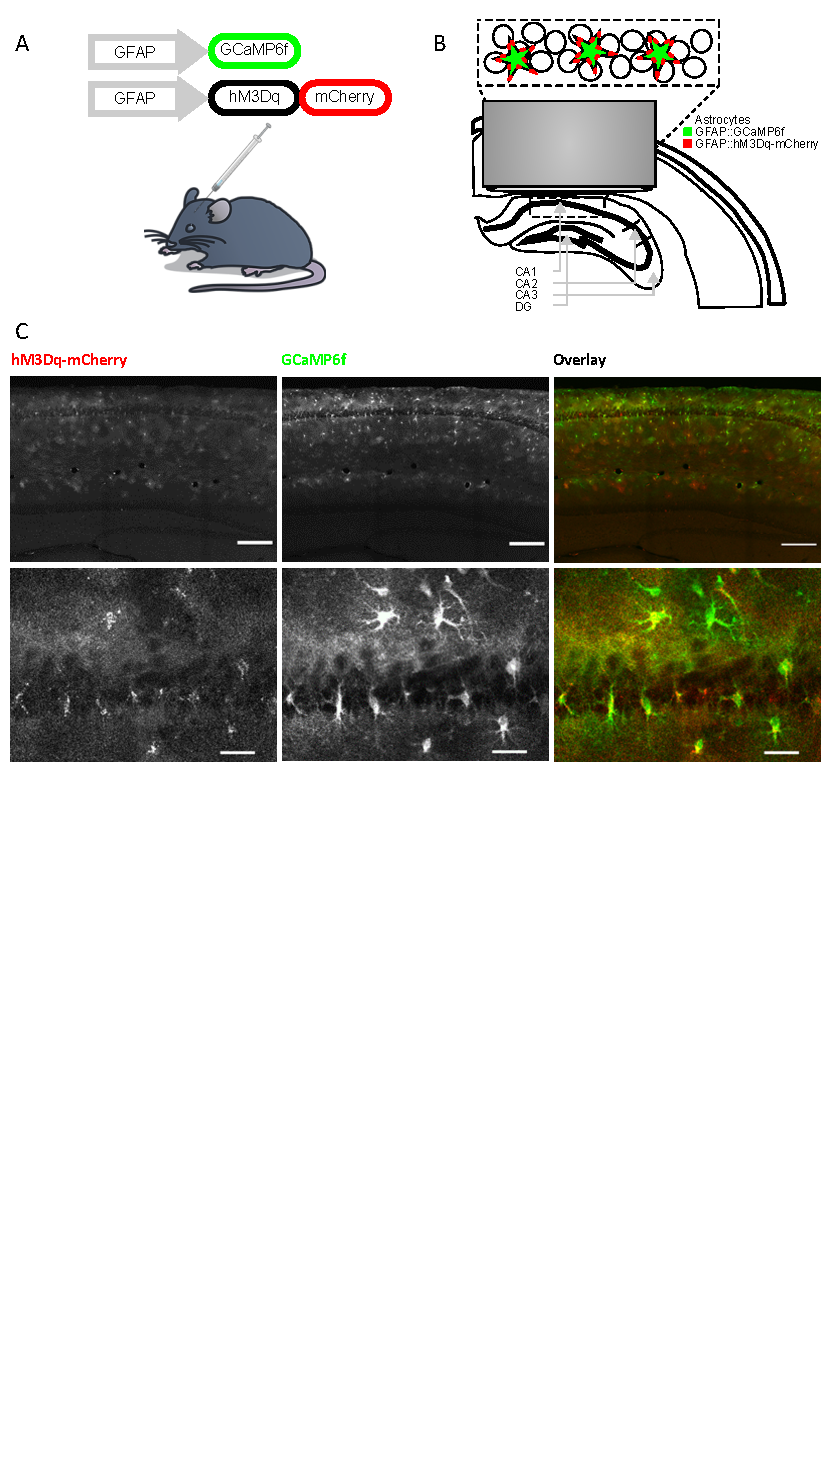
\includegraphics[trim={0 320 0 0},clip,width=\textwidth]{Figures/Chapter4/mcherry_gcamp_expression.pdf}
    \caption[Viral strategy to investigate astrocytic calcium signaling upon pharmacogenetic intervention.]{\textbf{Viral strategy to investigate astrocytic calcium signaling upon pharmacogenetic intervention.} 
    A) Adult mice were injected with two serotype 5 rAAV.
    One vector encoded for the genetically encoded calcium indicator GCaMP6f.
    The second vector encoded for the fusion construct hM3Dq-mCherry.
    Both constructs were under the control of the astrocyte-specific promoter GFAP.
    Injection was performed using stereotaxic coordinates to target the right hippocampus.
    B) Schematic of the chronic optical access to hippocampal CA1 area. 
    Optical access was granted by the implant of a chornic hippocampal imaging window above CA1 area. 
    C) Confocal micrographs of CA1 area of mice transduced with GFAP::GCaMP6f and GFAP::hM3Dq-mCherry rAAVs. 
    Images show astrocytes-specific co-expression of the two viral constructs in large volumes of hippocampal CA1 area. 
    Top: low magnification micrographs highlighting infection diffusion (scale $= 200\ \mu m$). 
    Bottom: high magnification micrographs showing in detail that the vast majority of astrocytes expressed simultaneously hM3Dq-mCherry fusion protein and GCaMP6f indicator (scale $= 30\ \mu m$).}
    \label{fig:chap4:mcherry_gcamp_expression}
\end{figure}
Viral delivery was performed via stereotaxic injection into the CA1 area of the right hippocampus (Figure \ref{fig:chap4:mcherry_dq_expression}B).
This strategy resulted in the vast majority of CA1 astrocytes expressing the hM3Dq fusion construct, as verified by immunolabeling with the astrocyte specific marker $S100\beta$ (Figure \ref{fig:chap4:mcherry_dq_expression}C).
\begin{figure}[h!]
    \centering
    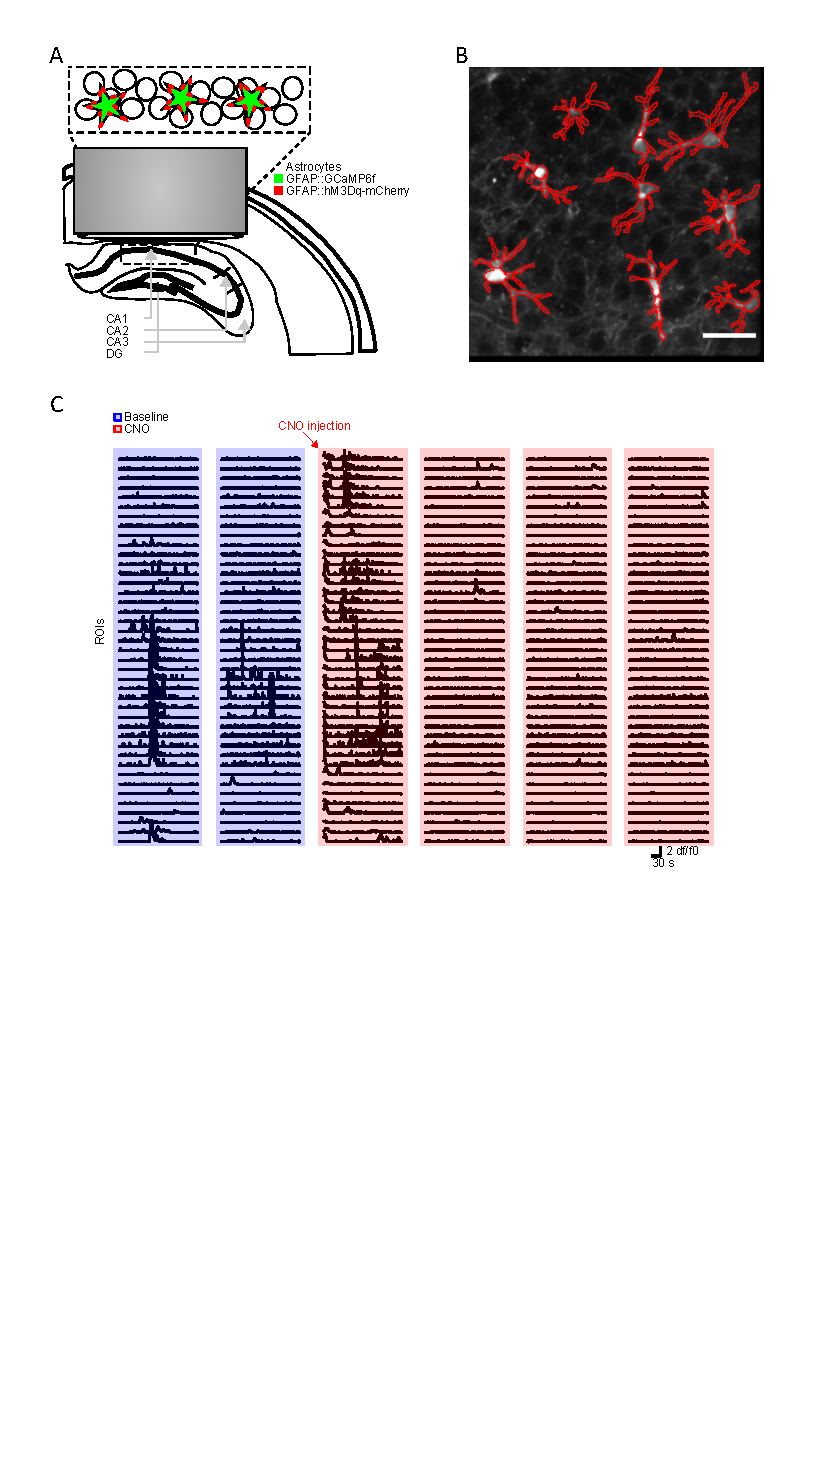
\includegraphics[trim={0 280 0 0},clip,width=\textwidth]{Figures/Chapter4/CNO_effect_calcium.pdf}
    \caption[In vivo two-photon calcium imaging of CA1 astrocytes during pharmacogenetic intervention.]{\textbf{In vivo two-photon calcium imaging of CA1 astrocytes during pharmacogenetic intervention.} 
    A) Schematic of the optical preparation to perform two-photon calcium imaging in astrocytes expressing the genetically encoded calcium indicator GCaMP6f and the pharmacogenetic actuator hM3Dq. 
    B) Temporal median projection of a sample field of view (scale $30\ \mu m$, field of view size approx $160\ \mu m^2$). 
    Astrocytic regions of interest (ROIs) have been manually selected on the median projection according to anatomical structures. 
    C) Representative calcium traces for 40 out of 135 ROIs shown in panel B. We performed six$\cdot 248 s$ temporal serieses interleaved by $300 s$ intervals. 
    Blue shaded areas indicate baseline spontaneous activity. 
    CNO was administered intraperitoneally few seconds before starting the third temporal series (red arrow).  
    Red shaded areas indicate recordings under putative activation of hM3Dq-receptor. 
    CNO administration resulted in a sudden increase of calcium activity (third temporal series), followed by a phase in which astrocytes decreased their calcium dynamics (fourth to sixth temporal series).}
    \label{fig:chap4:CNO_effect_calcium}
\end{figure}
Importantly, within the virally transduced region, hM3Dq expression was limited to the astrocytic outer membranes (Figure \ref{fig:chap4:mcherry_dq_expression}C).
\begin{figure}[h!]
    \centering
    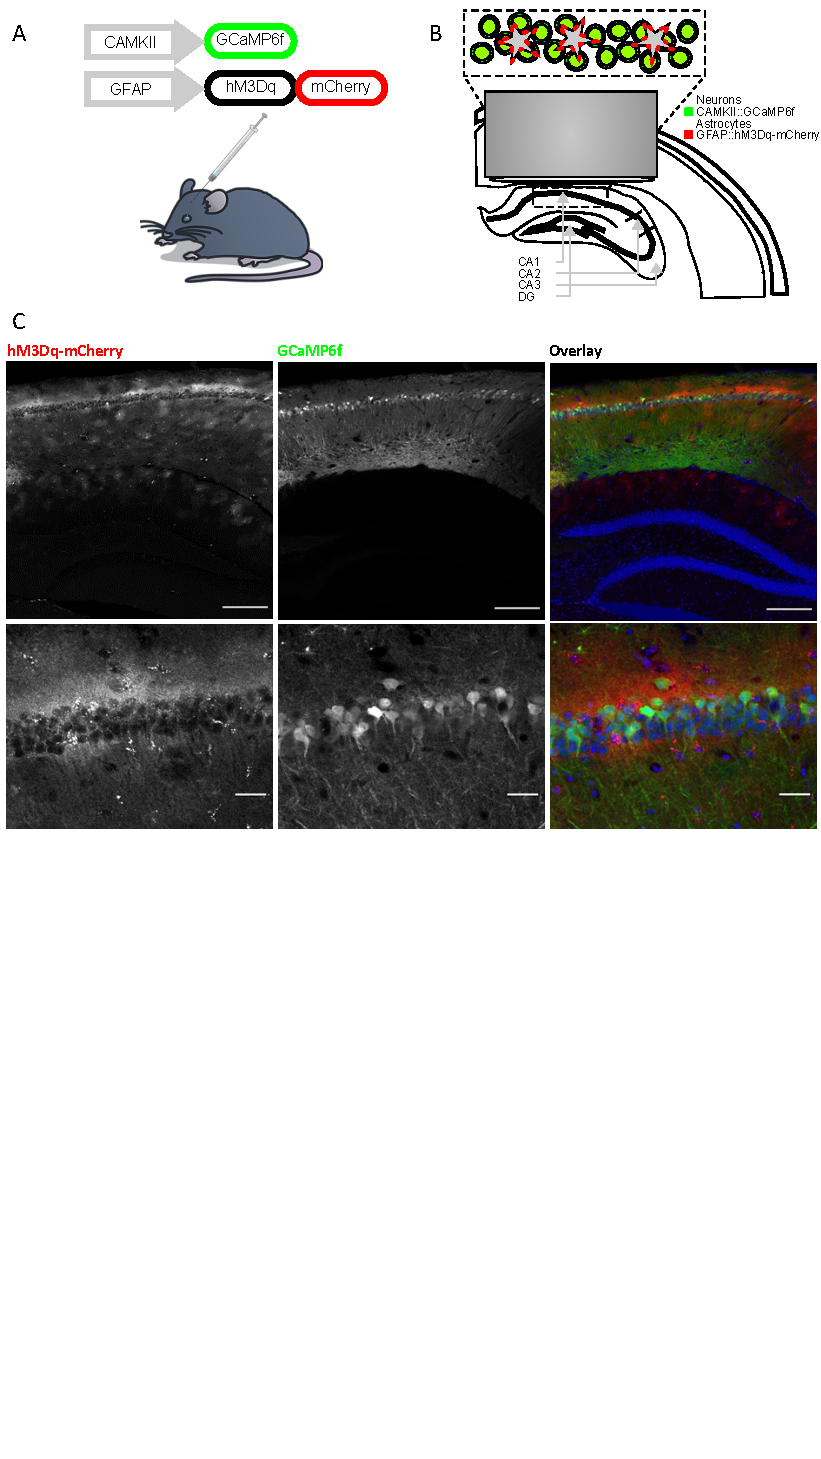
\includegraphics[trim={0 300 0 0},clip,width=\textwidth]{Figures/Chapter4/Pedro_fig5.pdf}
    \caption[Viral strategy to investigate neuronal calcium signaling under pharmacogenetic manipulation of astrocytic calcium signaling.]{\textbf{Viral strategy to investigate neuronal calcium signaling under pharmacogenetic manipulation of astrocytic calcium signaling.} 
    A) Adult mice were injected with two viral vectors: i) one vector encoded for the genetically encoded calcium indicator GCaMP6f under the control of the neuronal specific promoter CAMKII; ii) serotype 5 rAAV encoding for the fusion construct hM3Dq-mCherry. 
    Injection was performed using stereotaxic coordinates to target the right hippocampus. 
    B) Schematic of the chronic optical access to hippocampal CA1 area. 
    Optical access was granted by the implant of a chornic hippocampal imaging window above CA1 area. 
    C) Confocal micrographs of CA1 area of mice transduced with CAMKII::GCaMP6f and GFAP::hM3Dq-mCherry rAAVs. 
    Images show astrocytes-specific expression of hM3Dq-mCherry fusion construct and neuronal specific expression of GCaMP6f. 
    Infection spread in large volumes of hippocampal CA1 area. 
    Top: low magnification micrographs highlighting infection diffusion (scale $= 200\ \mu m$). 
    Bottom: high magnification micrographs showing in detail astrocytic expression of hM3Dq-mCherry fusion protein and neuronal specific expression of GCaMP6f indicator (scale $= 30\ \mu m$).}
    \label{fig:chap4:Pedro_fig5}
\end{figure}

To validate the effects of hM3Dq activation in vivo, we simultaneously labeled astrocytes with GCaMP6f and hM3Dq-mCherry. 
Coexpression was obtained by coinjection of two viral constructs under the control of the GFAP promoter and packaging in pseudotyped type-5 viral particles (Figure \ref{fig:chap4:mcherry_gcamp_expression}A-B). 
Under these conditions, coinfection was optimal, and it resulted in most hM3Dq-mCherry-expressing astrocytes being colabeled with GCaMP6f (Figure \ref{fig:chap4:mcherry_gcamp_expression}C).

We performed in vivo 2-photon calcium imaging in animals coexpressing hM3Dq and GCaMP6f. 
Optical access to the CA1 area of the hippocampus was obtained through a chronic hippocampal window [\cite{dombeck2010}] (Figure \ref{fig:chap4:CNO_effect_calcium}B). 
In anesthetized mice, we recorded the astrocytic calcium activity, which was characterized by heterogeneous dynamic signals involving astrocytic somata and processes (Figure \ref{fig:chap4:CNO_effect_calcium}C). 
We observed that CNO administration resulted in a sudden and synchronous increase in GCaMP6f fluorescence in astrocytes at the beginning of CNO application. 
This GCaMP6f signal increase was followed by a prolonged phase in which astrocytes showed decreased calcium dynamics (Figure \ref{fig:chap4:CNO_effect_calcium}C).

We used a viral delivery strategy to investigate the effects of the perturbation of astrocytic calcium dynamics on spatial information encoding in hippocampal neuronal cells. 
To monitor neuronal activity, we used a viral construct under the control of the CAMKII-promoter to express GCaMP6f in CA1 neurons (Figure \ref{fig:chap4:Pedro_fig5}A). 
CA1 astrocytes expressed hM3Dq-mCherry under the control of the GFAP promoter (Figure \ref{fig:chap4:Pedro_fig5}A). 
Within the virally transduced region, we reliably obtained GCaMP6f-labeled neurons and hM3Dq-mCherry-labeled astrocytes (Figure \ref{fig:chap4:Pedro_fig5}C).

% =========================================================== % 
%    Linear track section starts here                         %
% =========================================================== %

\section{Imaging neuronal place cells during pharmacogenetic manipulation of astrocytes in vivo: nonlongitudinal recordings}
\label{chap4:sec:3:linear_track}
To investigate the effects of the perturbation of astrocytic calcium dynamics on spatial information encoding in hippocampal neuronal cells, we trained head-tethered mice to navigate in a unidirectional virtual environment while we performed two-photon functional imaging of neuronal cells (Figure \ref{fig:chap4:virtual_reality_setup}, \cite{saleem2018coherent}). 
We combined astrocyte-specific expression of hM3Dq and neuronal-specific expression of the genetically encoded calcium indicator GCaMP6f (Figure \ref{fig:chap4:FOV_example_setup}A) to capture hippocampal CA1 neuron activity.
\begin{figure}[h]
    \centering
    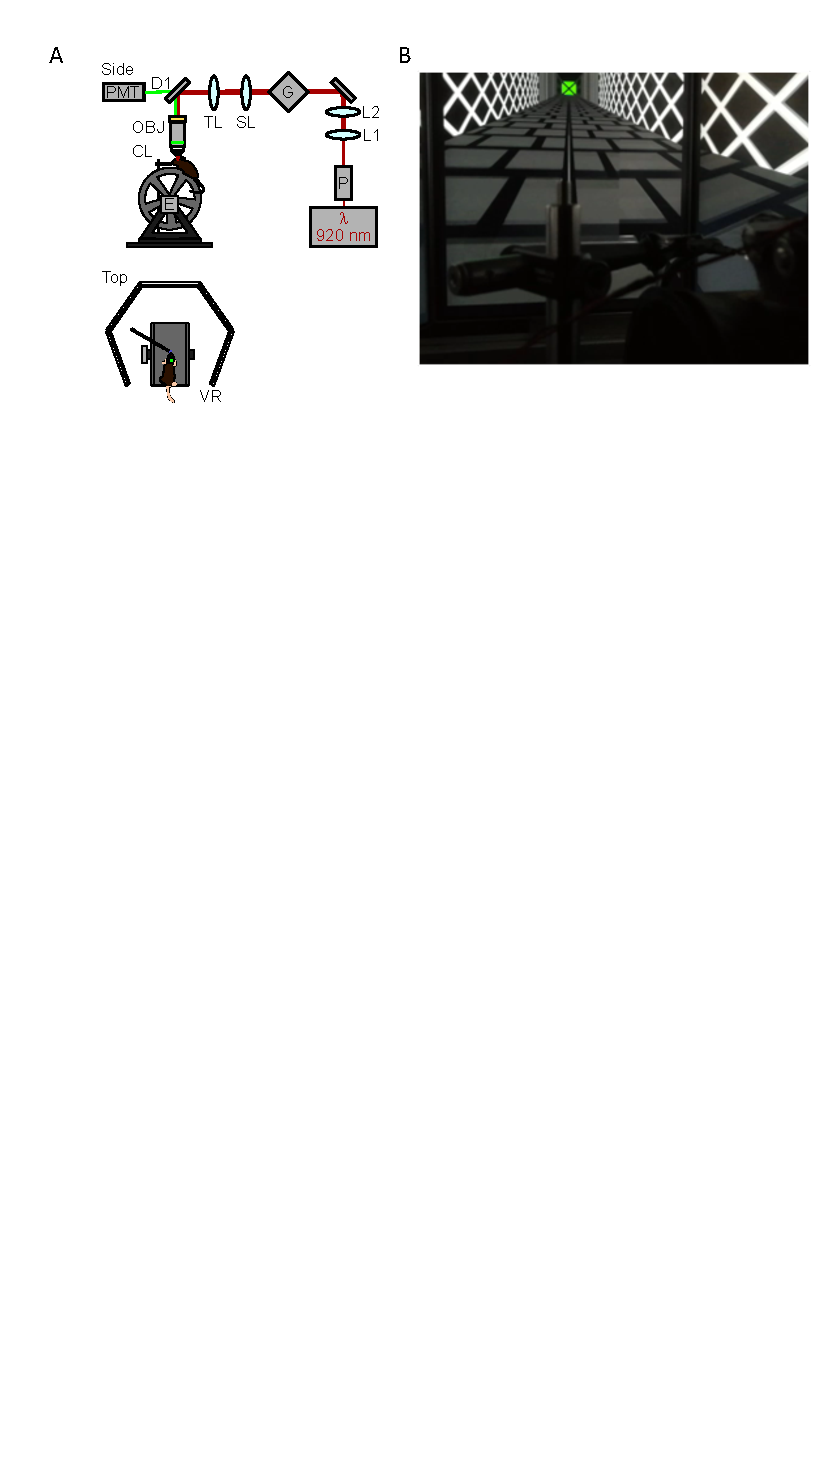
\includegraphics[trim={0 500 0 0},clip,width=\textwidth]{Figures/Chapter4/virtual_reality_setup.pdf}
    \caption[Two photon functional imaging during virtual spatial navigation.]{\textbf{Two photon functional imaging during virtual spatial navigation.} 
    A) Schematic of virtual reality and imaging setup. Mice run along a virtual corridor provided with visual features (B), at the end of each run they get teleported back to the beginning of the track. 
    B) Sample of mouse visuals from the beginning of the linear track.}
    \label{fig:chap4:virtual_reality_setup}
\end{figure}

To extract the calcium activity traces of neurons in CA1, we first computed the median  temporal projection of the field of view on motion-corrected two-photon calcium imaging t-series (Figure \ref{fig:chap4:segmentation_traces_2p}A top). 
We used CITE-on (see methods \ref{chap3:sec:4:segmentation} and appendix \ref{CITE-On}), which is a deep learning-based algorithm for fast segmentation of neurons in two-photon imaging data (see appendix \ref{CITE-On}), to detect neuronal cells in the median projections, obtaining rectangular regions of interest (bounding boxes) tightly surrounding putative neuronal somas (Figure \ref{fig:chap4:segmentation_traces_2p}A bottom). 
To perform segmentation on bounding boxes, we used a spatially confined version of the nonnegative matrix factorization algorithm (seeded-CaImAn, \cite{giovannucci2019}). 
Seeded-CaImAn was initialized on each bounding box, yielding precise segmentation of the putative neuronal source and its respective calcium activity trace.
\begin{figure}[h!]
    \centering
    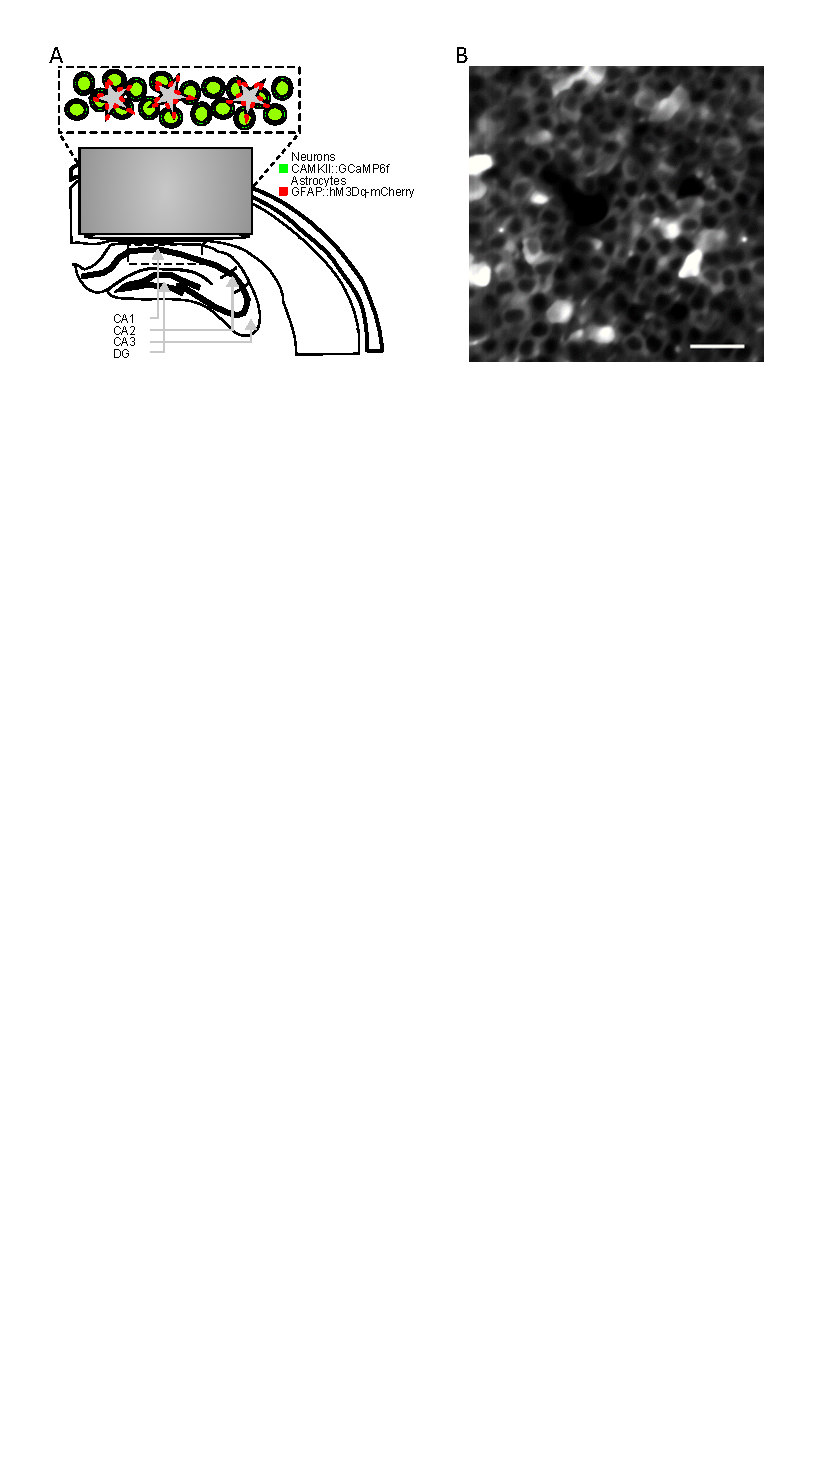
\includegraphics[trim={0 530 0 0},clip,width=\textwidth]{Figures/Chapter4/FOV_example_setup.pdf}
    \caption[In vivo two-photon calcium imaging of CA1 neurons and pharmacogenetic astrocytic manipulation during virtual navigation.]{\textbf{In vivo two-photon calcium imaging of CA1 neurons and pharmacogenetic astrocytic manipulation during virtual navigation.} 
    A) Schematic of the optical preparation to perform two-photon calcium imaging in CA1 neurons labeled with the genetically encoded calcium indicator GCaMP6f while astrocytic activity was manipulated using the pharmacogenetic actuator hM3Dq. 
    B) Temporal median projection of a sample field of view (scale $= 30\ \mu m$, field of view size approx $160\ \mu m^2$).}
    \label{fig:chap4:FOV_example_setup}
\end{figure}
For each calcium trace, $\Delta F/F_0$ was computed (Figure \ref{fig:chap4:segmentation_traces_2p}B top), and calcium events were detected with a threshold criterion based on the $\Delta F/F_0$ trace (see Methods \ref{chap3:sec:6:event_det}).
To build the \textit{event trace}, all time instants that did not belong to an event were set to zero. 
Calcium events corresponded to above-threshold calcium transients generated by putative neuronal spikes (Figure \ref{fig:chap4:segmentation_traces_2p}B zoom-in).
\begin{figure}[h]
    \centering
    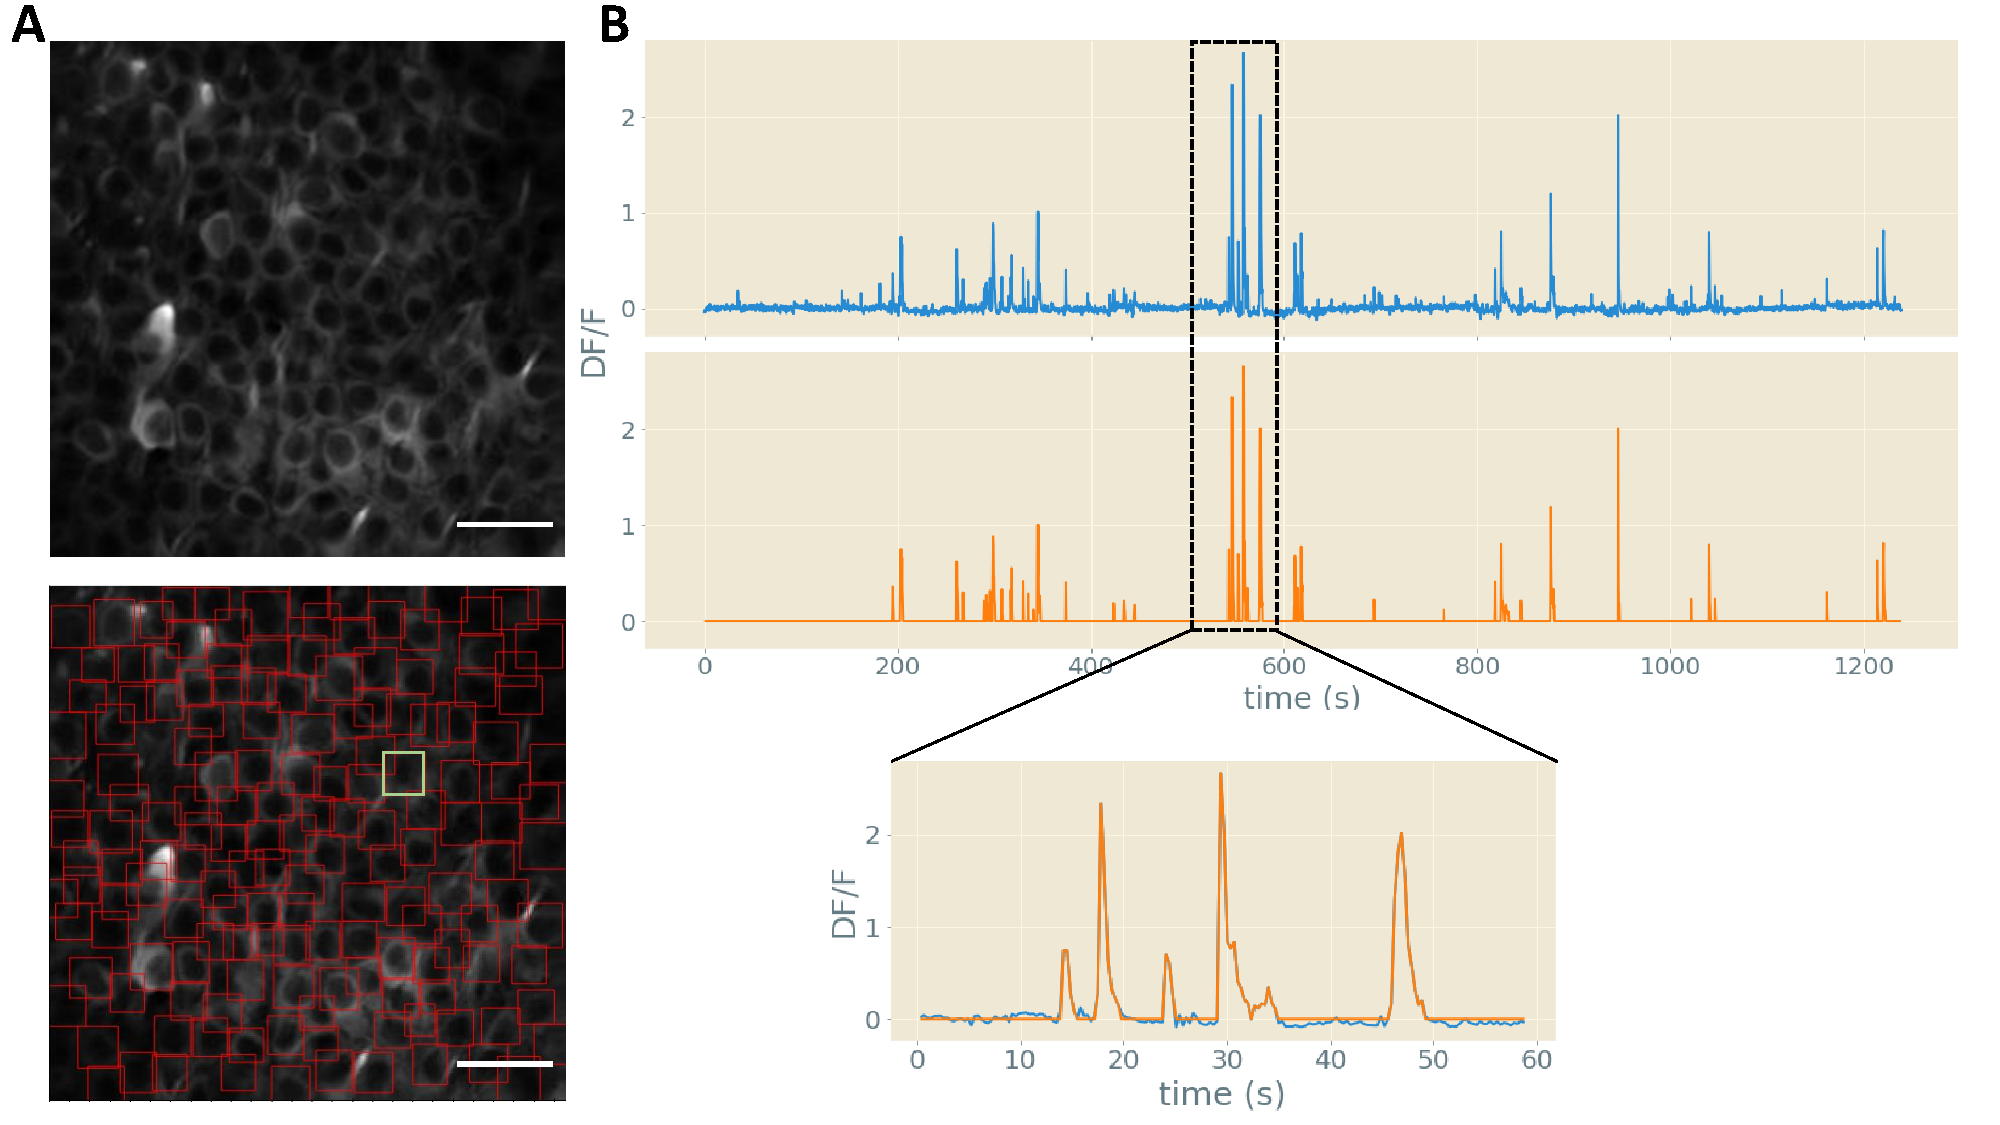
\includegraphics[trim={0 0 150 0},clip,width=\textwidth]{Figures/Chapter4/segmentation_traces_2p.pdf}
    \caption[Segmentation and trace extraction of 2-photon imaging data]{\textbf{Segmentation and trace extraction of 2-photon imaging data.} A) Median projection of a representative recording of CA1 neurons (top) and the detected boxes segmented with CITE-on in red (bottom) (scale $30\ \mu m$, field of view size approx $160\ \mu m^2$).
    B) Representative $\Delta F/F_0$ trace extracted using seeded-CaImAn in blue, and the event trace in orange. A zoom of one minute of recording is shown in the bottom panel. The trace corresponds to the green box in bottom panel A.}
    \label{fig:chap4:segmentation_traces_2p}
\end{figure}

To study how neuronal activity is related to the animal position, calcium traces from neuronal populations were analyzed in the context of mice running in a 1-dimensional virtual corridor (or linear track).
$\Delta F/F_0$ traces were averaged across trials (runs in the linear track) to obtain the average calcium intensity as a function of position in the track, which is hereafter termed the \textit{response profile}.
Response profiles were modeled as a sum of gaussians with different centers, widths (or sigmas), and amplitudes (see methods \ref{chap3:sec:7:subsec1:PF_and_response_profiles}). 
For each response profile, we considered the gaussian component with the highest amplitude as the \textit{response field} (RF). 
Intuitively, this is the fraction of the linear track in which each cell showed the highest average activity.
Five representative response profiles are shown in Figure \ref{fig:chap4:pf_gaussian_fitting}, together with the corresponding response field functions (gray dashed lines) and response field \textit{widths} (gray shadowed areas).
Modeling, fitting, and estimation of the centers and widths of response profiles were performed for all detected regions of interest.

We studied how neuronal activity is related to the animal position in the linear track as a function of the pharmacogenetic perturbation of astrocytic calcium activity.
In detail, 20 recordings from 7 animals were analyzed. 
Animals received an intraperitoneal injection of either saline solution (control; $n = 10$) or clozapine-n-oxyde (CNO; $n = 10$). 
Each injection required the animal to be removed from the two-photon microscope and subsequently repositioned and imaged. In this first dataset, imaging after injection was performed in a field of view that was not necessarily the same as that one monitored in the imaging session immediately right before CNO or saline injection. 
This meant that the same cell could not be monitored across conditions (nonlongitudinal recordings).
One recording of each treatment (CNO or saline) was analyzed for each animal, with the exception of animal \textit{0001} (2 recordings for each condition) and animal \textit{0002} (3 recordings for each condition).
On average, 109 cells were detected \textit{per} FOV (min 50; max 165), resulting in a total of 2193 cells studied.
Further imaging sessions were performed in all animals, but they were discarded due to technical issues (e.g., large movement artifacts). 
\begin{SCfigure}[][h]
    %\centering
    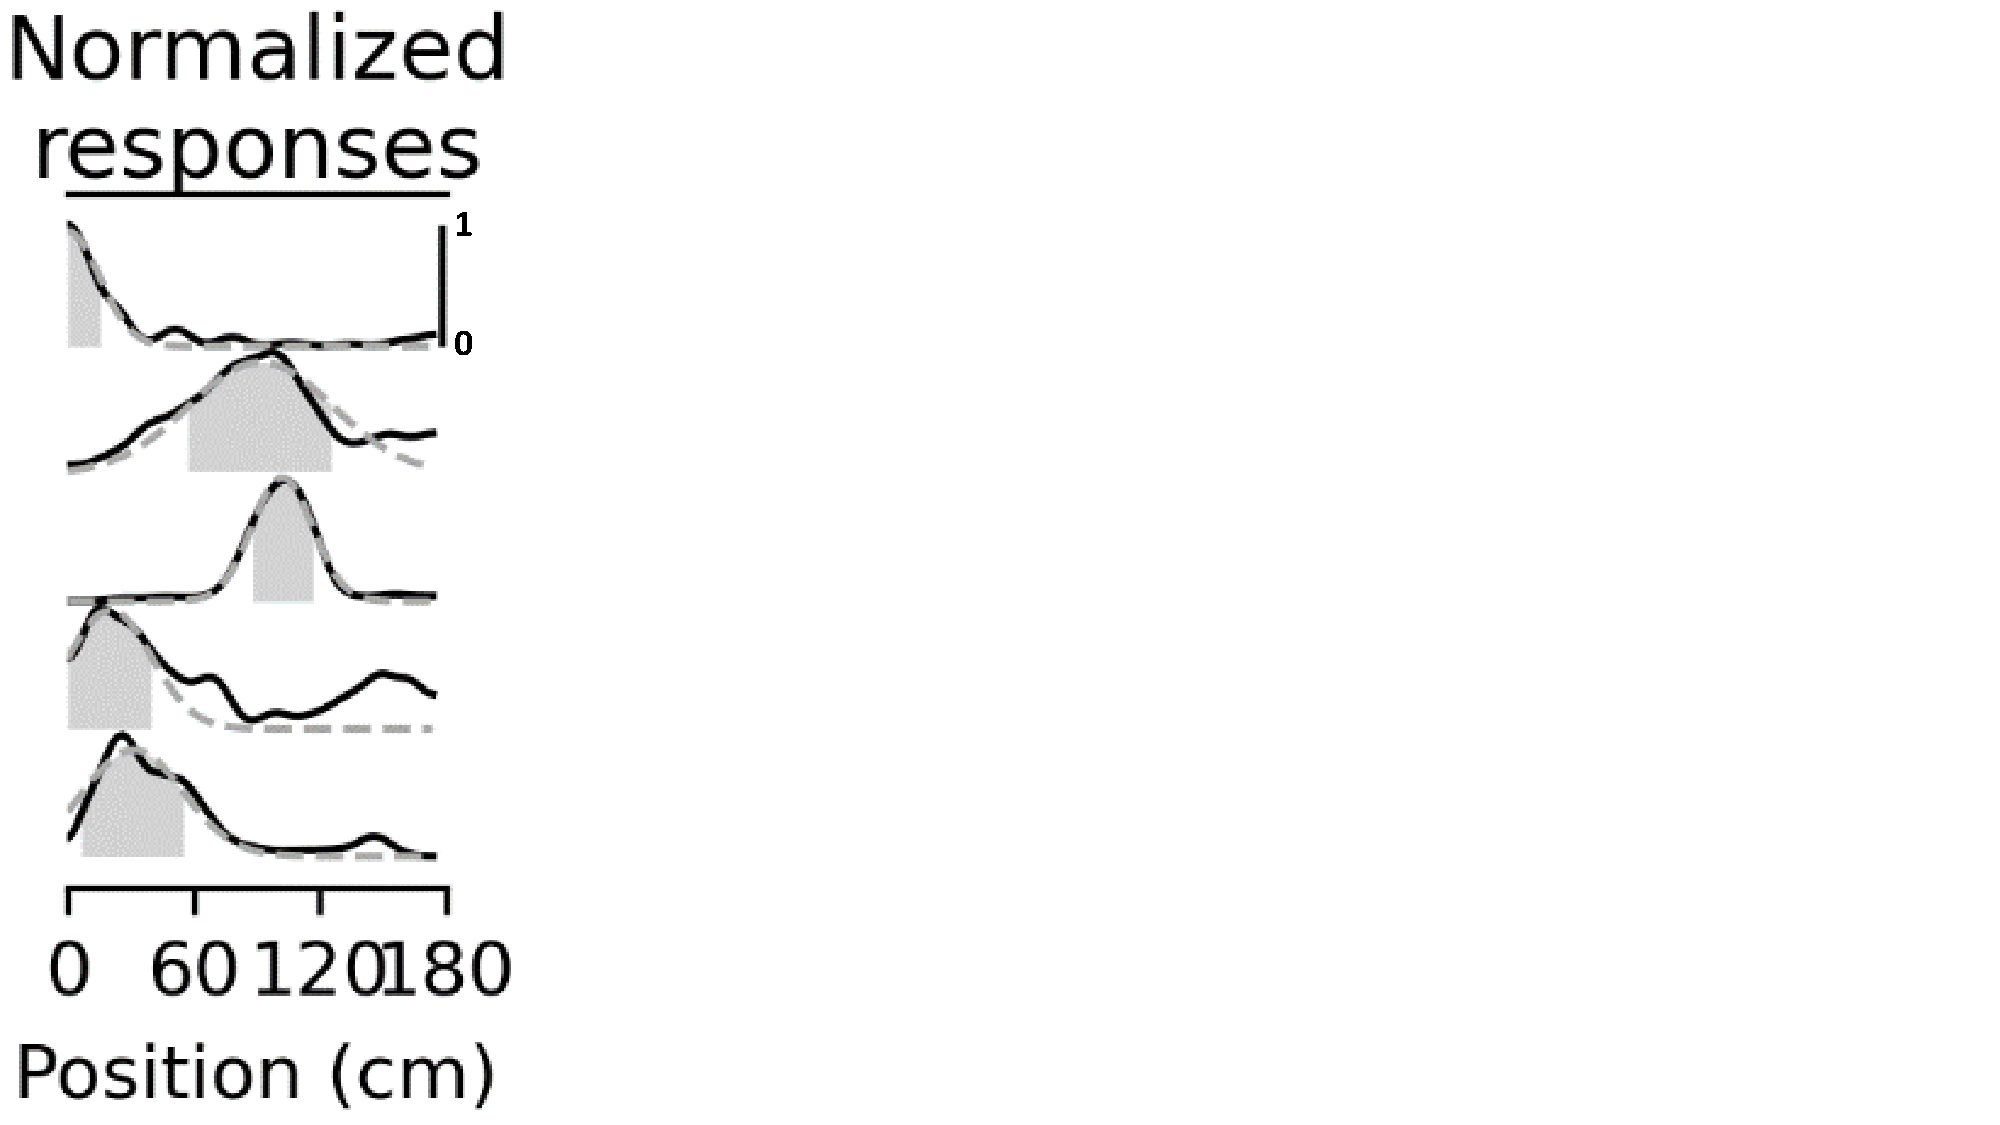
\includegraphics[trim={0 0 710 0},clip,width=.3\textwidth]{Figures/Chapter4/pf_gaussian_fitting.pdf}
    \caption[Place field estimation]{\textbf{Place field estimation.} Representative examples of the normalized response profiles of five cells (black line) with their gaussian fit (dotted gray lines) to estimate place fields. 
    The gray-shadowed areas show the width of the place fields, which is defined as $\mu \pm \sigma$, with $\mu$ and $\sigma$ being the mean and standard deviation of the fit, respectively.}
    \label{fig:chap4:pf_gaussian_fitting}
\end{SCfigure}

We then applied an information theory approach (see introduction) to compute the amount of spatial information contained in each identified neuron. 
More specifically, we computed the Shannon entropy (eq. \ref{eqn:entropy} of the introduction) and then the mutual information (eq. \ref{eqn:mutualinfo2} of the introduction) about the spatial variable contained in the calcium signal extracted from each identified neuron. 
For each neuron, we then calculated whether the amount of spatial information was significant by comparing the mutual information of that cell with a surrogate distribution of mutual information values (see methods \ref{chap3:sec:7:subsec2:pc_analysis}).
In figure \ref{fig:chap4:snake_plot_2p}, we show the normalized calcium responses of all neurons with significant information content about space (see methods \ref{chap3:sec:7:subsec2:pc_analysis}) ordered according to the position of the center of the response field in increasing order.
The left panel shows recordings after saline injection, and the right panel shows recordings after CNO injection (283 and 329 informative  ROIs out  of  1192 and 1001 total, respectively). 
In both cases, the place field of neurons spans the whole virtual corridor, allowing for complete mapping of the space, regardless of treatment. 
In the case of place cells, the centers $\mu$ and widths $\sigma$ of the principal gaussian component had a straightforward interpretation as the center and width of the place field. 
For cells without significant information content about space, the $\mu$ and $\sigma$ parameters give us information about where the animal responded maximally on average and how spread out the response was in space (Figure \ref{fig:chap4:pf_gaussian_fitting}).
This information is relevant when trying to uncover the effects of alterations in calcium activity in astrocytes on neuronal networks in the hippocampus beyond place cell encoding. 
\begin{SCfigure}[][h]
    \centering
    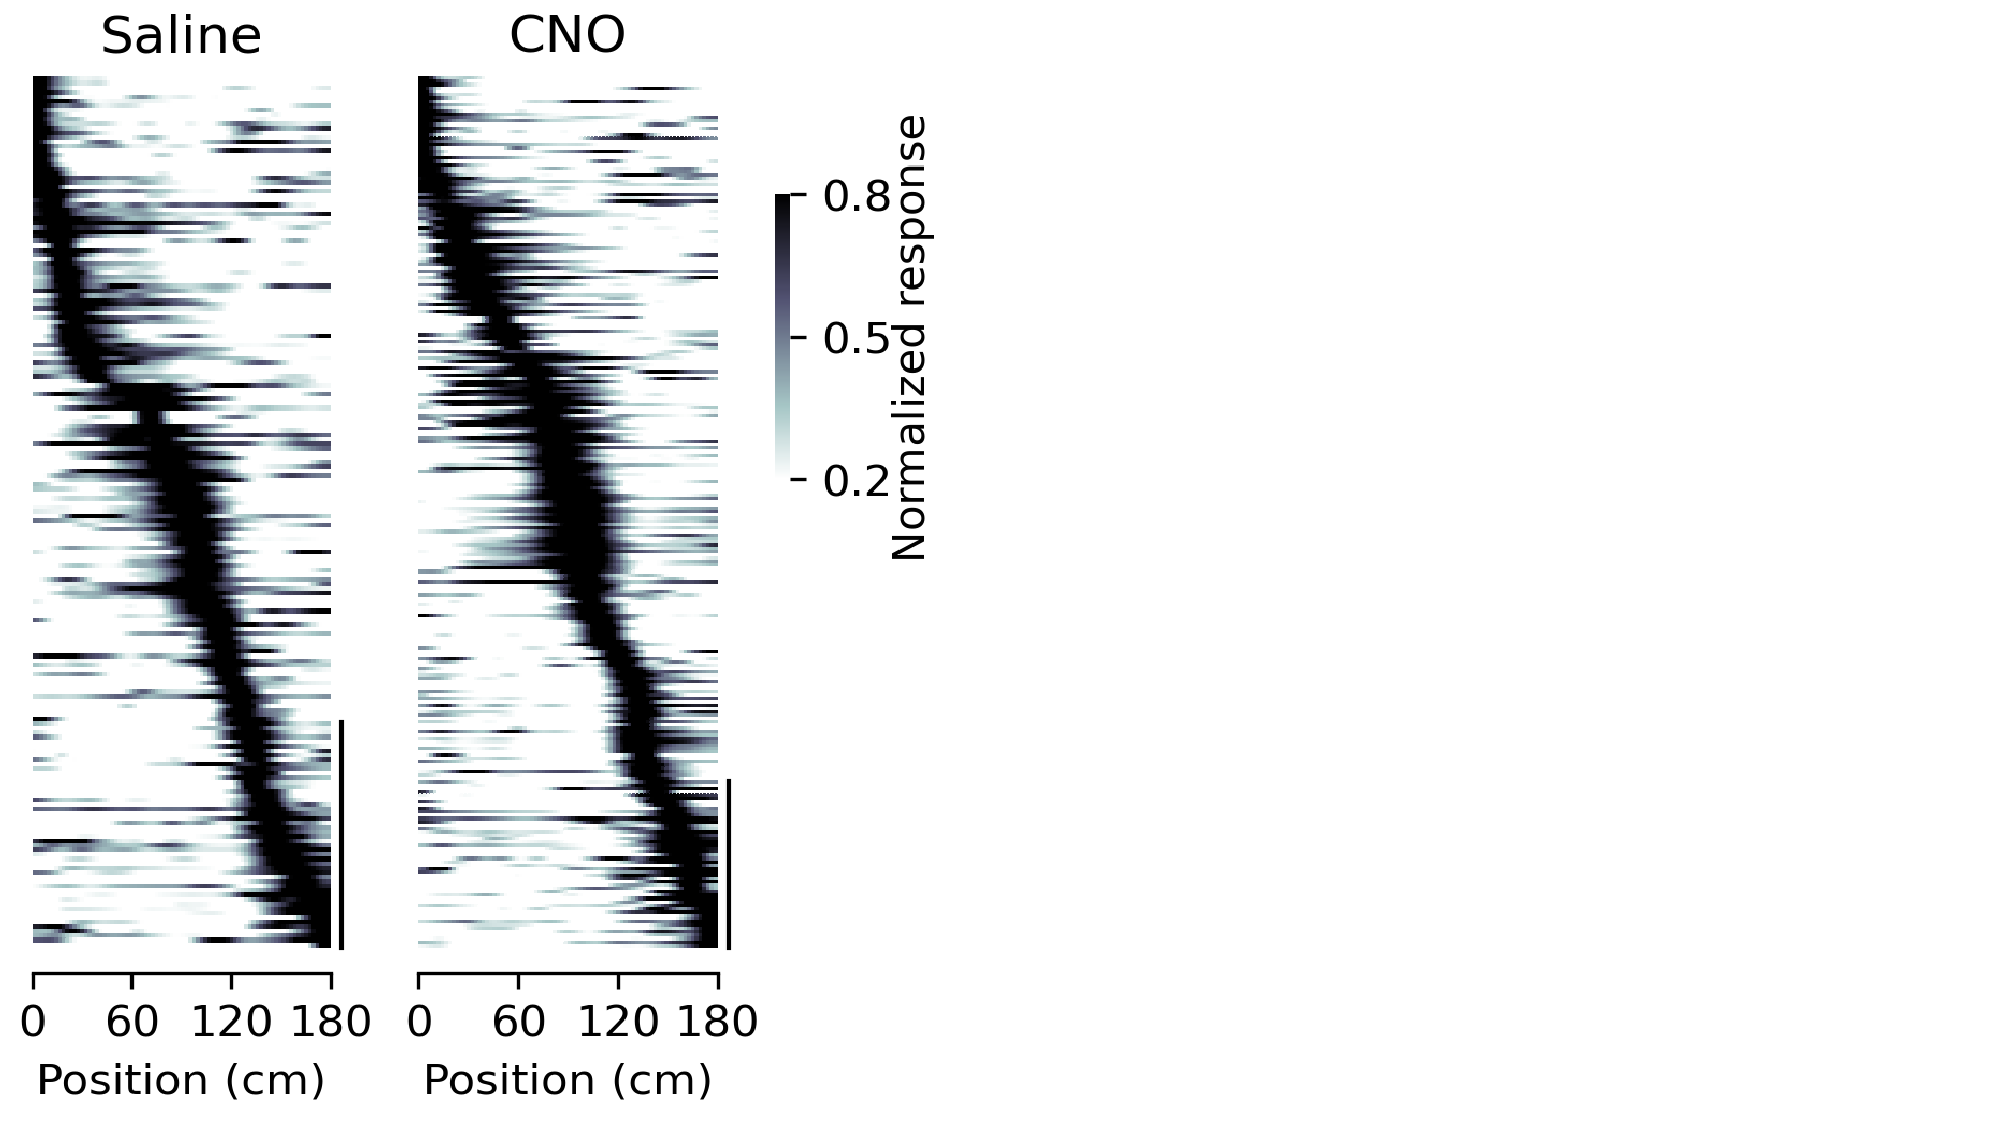
\includegraphics[trim={0 0 500 0},clip,width=0.5\textwidth]{Figures/Chapter4/snake_plots_2p.pdf}
    \caption[Normalized calcium responses as a function of position for neurons that contain significant amount of spatial information]{\textbf{Normalized calcium responses as a function of position for neurons that contain significant amount of spatial information.} 
    Left panel, responses from recordings in which the animal was injected with saline solution (n = 283 informative ROIs out of 1192 total ROIs, 10 imaging sessions from 7 animals). 
    Right panel, responses from recordings in which the animal was injected with CNO solution (n = 329 informative ROIs out of 1001 total ROIs, 10 imaging sessions from 7 animals). 
    Responses are ordered according to the position of the center of the response field (from minimum to maximum). 
    As described in the results, the FOV which was imaged in the saline condition was different from the one recorded in the CNO condition (nonlongitudinal recordings).}
    \label{fig:chap4:snake_plot_2p}
\end{SCfigure}

To correct for biases in MI values, we first computed the $NsR$ parameter (see methods \ref{chap3:sec:7:subsec3:bias_correction}) for all recordings as a function of the number of response (calcium activity) and stimulus (position) bins (Figure \ref{fig:chap4:bias_corr_2p}A).
$NsR=3$ was considered a threshold above which description of the variables with respect to the number of trials was acceptable (red squares).
We then calculated the average mutual information values after bias subtraction for different configurations of binning (Figure \ref{fig:chap4:bias_corr_2p}B).
Bias-corrected mutual information values initially increased, then plateaued, and finally decreased with the number of spatial bins (Figure \ref{fig:chap4:MI_C_2p}C). 
In those cases, the bias term highly contributed to the mutual information value, and its subtraction resulted in a strong decrease in the bias-corrected MI values, which, in turn, was observed as a negative change in the slope of the curves. 
Separating the bias-corrected MI values for ROIs with significant information content from those without implies a clear split in the bias-corrected MI values (Figure \ref{fig:chap4:bias_corr_2p}C), with nonplace cells having distributions close to zero. 
Finally we calculated the average fractions of significant ROIs as a function of binning (Figure \ref{fig:chap4:bias_corr_2p}).
All four plots were performed and inspected separately for each data set, and appropriate binning was selected such that the level of description was as high as possible (higher number of bins) while having $SnR>3$ and maximized bias corrected MI values (before the change in slope).  
\begin{figure}[h]
    \centering
    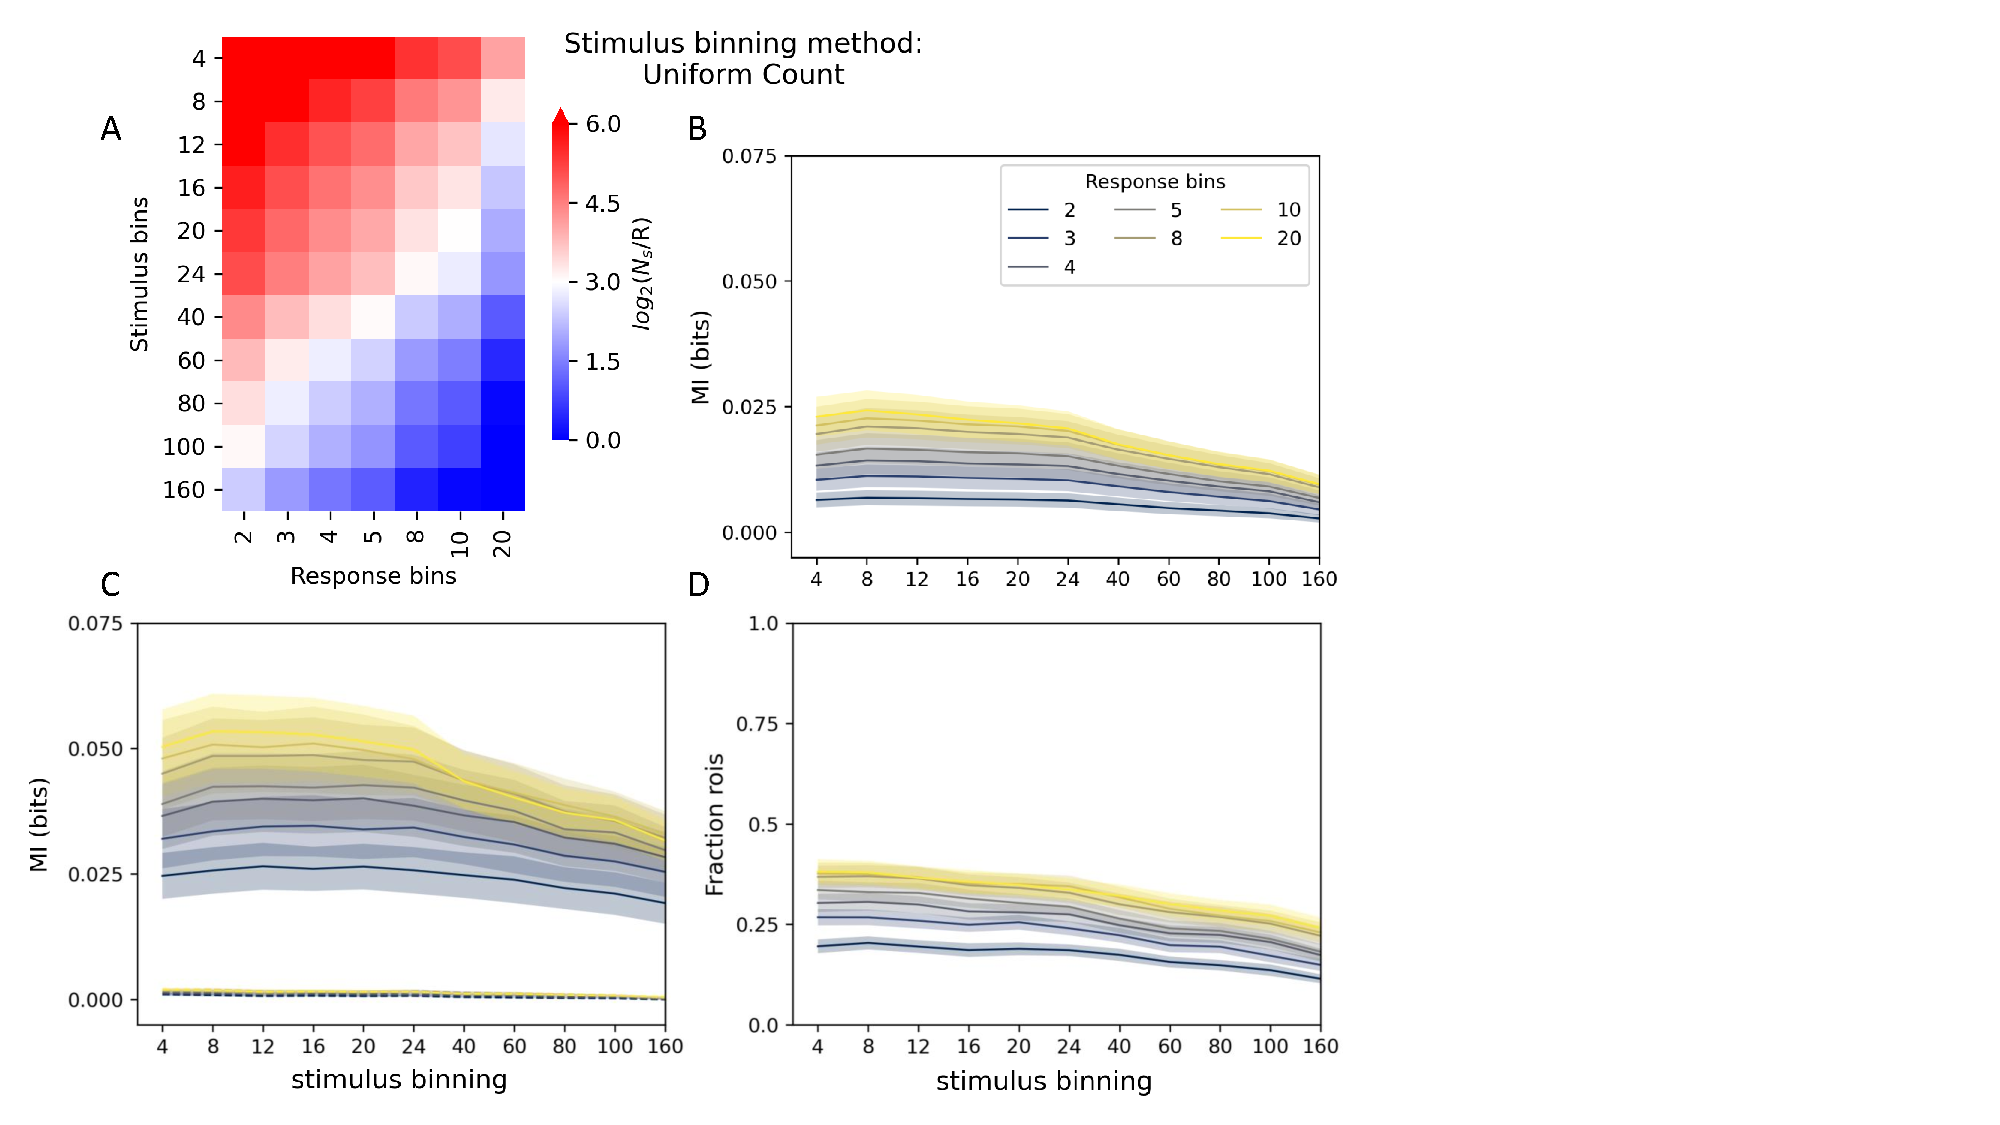
\includegraphics[trim={0 0 300 0},clip,width=\textwidth]{Figures/Chapter4/bias_correction_2p.pdf}
    \caption[Bias correction and binning selection for mutual informatin calculation]{\textbf{Bias correction and binning selection for mutual informatin calculation.} A) Matrix of log SnR parameter values for different response and stimulus binning. 
    log SnR = 3 was considered a adequate quality threshold. 
    B) Average bias corrected MI values as a function of spatial binning, each line corresponds to a different response binning. 
    C) Bias corrected MI values as in (A) separated in cells with significant information content (filled lines) and without (dotted lines). 
    D) Fraction of ROIs with significant information content as a function of binning as in (A).}
    \label{fig:chap4:bias_corr_2p}
\end{figure}

To study the effect of CNO injection on the information content about animal position in CA1 neuronal calcium activity, we calculated the bias-corrected MI for all cells (Figure \ref{fig:chap4:MI_C_2p}).
We first compared the distribution of MI values after saline or CNO injection for each animal.
Boxplots and statistical testing are reported in each of the first 7 panels.
Here, both place cells and nonspatial encoding cells are pooled together; thus, the distributions are centered close to zero and heavy tailed towards positive values. 
Although not all animals had significantly different MI distributions (Mann-Whitney U test was performed in each case), when comparing averages across animals, we observed a significant increase in information content in experiments following CNO injection (Wilcoxon paired test, $p=0.028$, Figure \ref{fig:chap4:MI_C_2p} bottom right panel).

Variability between data from different animals could bring differences across distributions that might mask the effect of CNO treatment. 
To account for this effect, we used a linear mixed effect (LME) model, taking the treatment (CNO or saline injection) as a fixed effect and the animal identity as a random effect (see methods \ref{chap3:sec:8:stats}).
In each case, we compared 2 models-one with a random intercept (LME1, eq. \ref{eqn:LMEM1}) and another with a random intercept and a random slope (LME2, eq. \ref{eqn:LMEM2}). 
If the model that included the random slope explained significantly more variance, then this model was preferred (ANOVA test for model comparison).
If, in contrast, the models were not significantly different, the simpler test was used.
When comparing all cells from all animals, the LME2 model was used (LME2 explained significantly more variance than did LME1, using ANOVA for model comparison, $p=6\cdot 10^{-4}$).
The fitted slope of the LME2 model was -0.01 (negative values implied a decrease in information for saline conditions), and the effect of the treatment was found to be statistically significant (Type II Wald chi-square tests, $p=0.005$).
\begin{figure}[h]
    \centering
    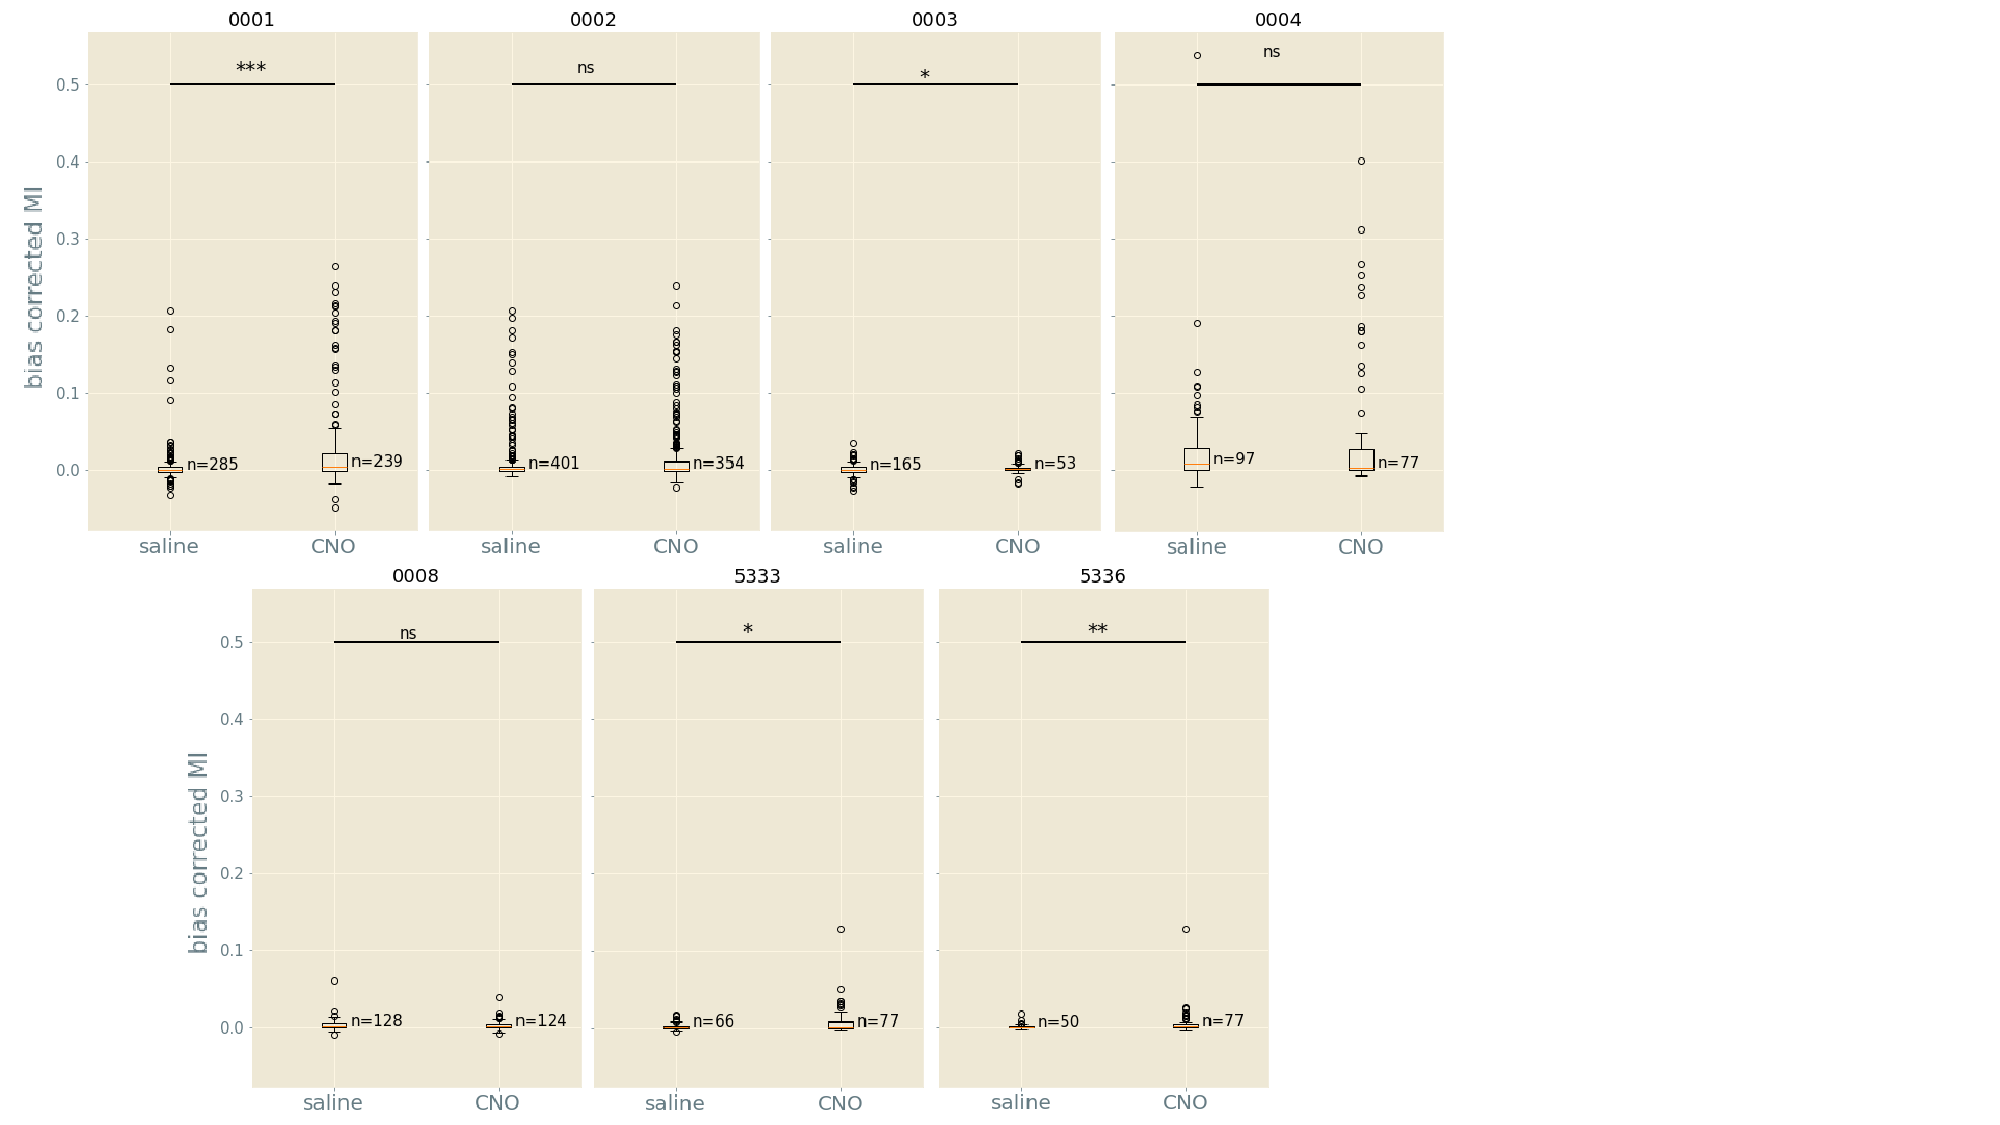
\includegraphics[trim={0 0 160 0}, clip, width=\textwidth]{Figures/Chapter4/MI_C_all_cells_2p.pdf}
    \caption[Higher information content about animals position in neuronal cells after CNO application]{\textbf{Higher information content about animals position in neuronal cells after CNO application.} 
    Box plots of bias corrected MI values for each animal (each panel represents an animal) after saline or CNO injection. 
    Not all animals have significantly different information content, but they do when averaged together (bottom right panel, Wilcoxon paired test, $p = 0.028$).}
    \label{fig:chap4:MI_C_2p}
\end{figure}

Because place cells contributed the most to the information content about the animal position, we asked whether changes in MI values were observed when comparing CNO and saline conditions and when only place cells were considered. 
We fitted LME1 considering only place cells (note that this is a test on a subsample of the previous distribution), obtaining a slope of -0.026 and an even more significant effect ($p=4 \cdot 10^{-6}$).
These results showed that the increase in the information content after CNO injection was higher when considering only place cells. 

To determine whether the effect could be influenced by the number of cells in each condition or whether CNO injection could have an effect on the number of cells detected, we compared the number of cells found in each condition (Figure \ref{fig:chap4:pc_quantification_2p} left panel) and found no significant difference (Wilcoxon paired test, $p=0.18$). 
We then quantified the number of place cells in each case (Figure \ref{fig:chap4:pc_quantification_2p} center panel) and found a small but significant increase after CNO injection (Wilcoxon paired test, $p=0.046$).
We then computed the ratio between the number of place cells and the total number of cells for each animal (Figure \ref{fig:chap4:pc_quantification_2p} right panel), which was found to be significantly higher for the CNO condition (Wilcoxon paired test, $p=0.017$).
\begin{figure}
    \centering
    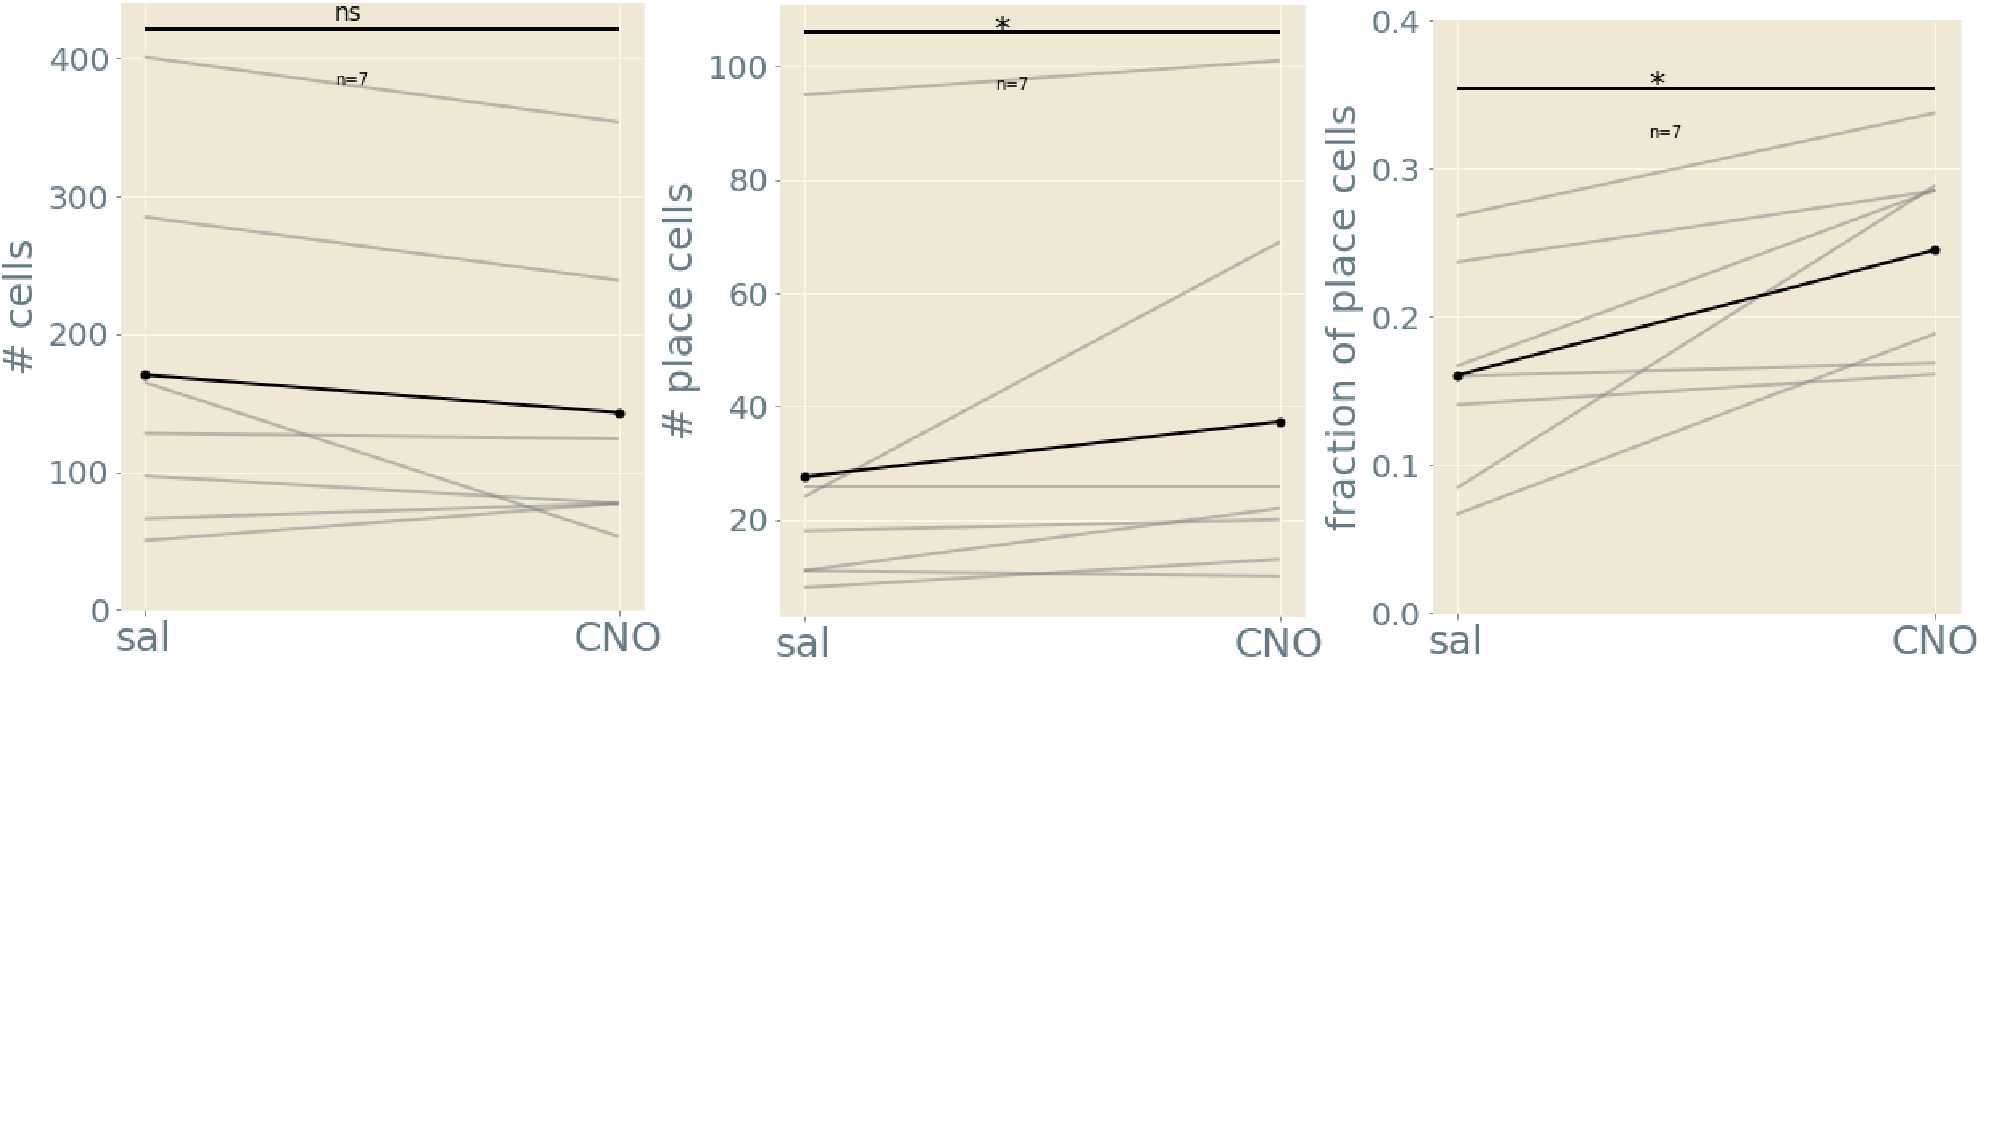
\includegraphics[trim={0 200 0 0},clip,width=\textwidth]{Figures/Chapter4/pc_quantification_2p.pdf}
    \caption[Increased number of place cells after CNO injection.]{\textbf{Increased number of place cells after CNO injection.} 
    The number of cells segmented per animal was not significantly different between conditions (Left panel, Wilcoxon paired test $p = 0.18$). 
    The number of place cells and fraction of place cells from the total number of cells was significantly higher following CNO injection (center panel $p=0.046$, and right panel $p=0.017$ respectively).}
    \label{fig:chap4:pc_quantification_2p}
\end{figure}

We further explored whether CNO application changed other properties of neuronal place cells.
We compared the center and width of response profiles and/or place fields after saline injection and after CNO injection (Figure \ref{fig:chap4:width_center_2p}).
When considering all cells, the response profile width was slightly but significantly higher after CNO injection (Figure \ref{fig:chap4:width_center_2p} top left panel, Kolmogorov-Smirnov test, $p=0.005$), as evidenced by a small shift to the right in the empirical distribution function (EDF).
The distributions of response profile centers were significantly different (Figure \ref{fig:chap4:width_center_2p} top right panel, $p=9\cdot 10^{-4}$).
We then considered the same comparisons for place field widths and centers, taking into account exclusively place cells (Figure \ref{fig:chap4:width_center_2p} bottom left and right panels, respectively). 
In both cases, the difference between distributions was not significant ($p=0.1$ for PF width and $p=0.13$ for PF centers). 

Taken together, these results suggest that CNO application, and, consequently, the modification of calcium signaling in astrocytes significantly affected the neuronal representation of space and the properties of neuronal place cells in the hippocampus of mice navigating in a unidimensional virtual corridor. 
\begin{figure}[h]
    \centering
    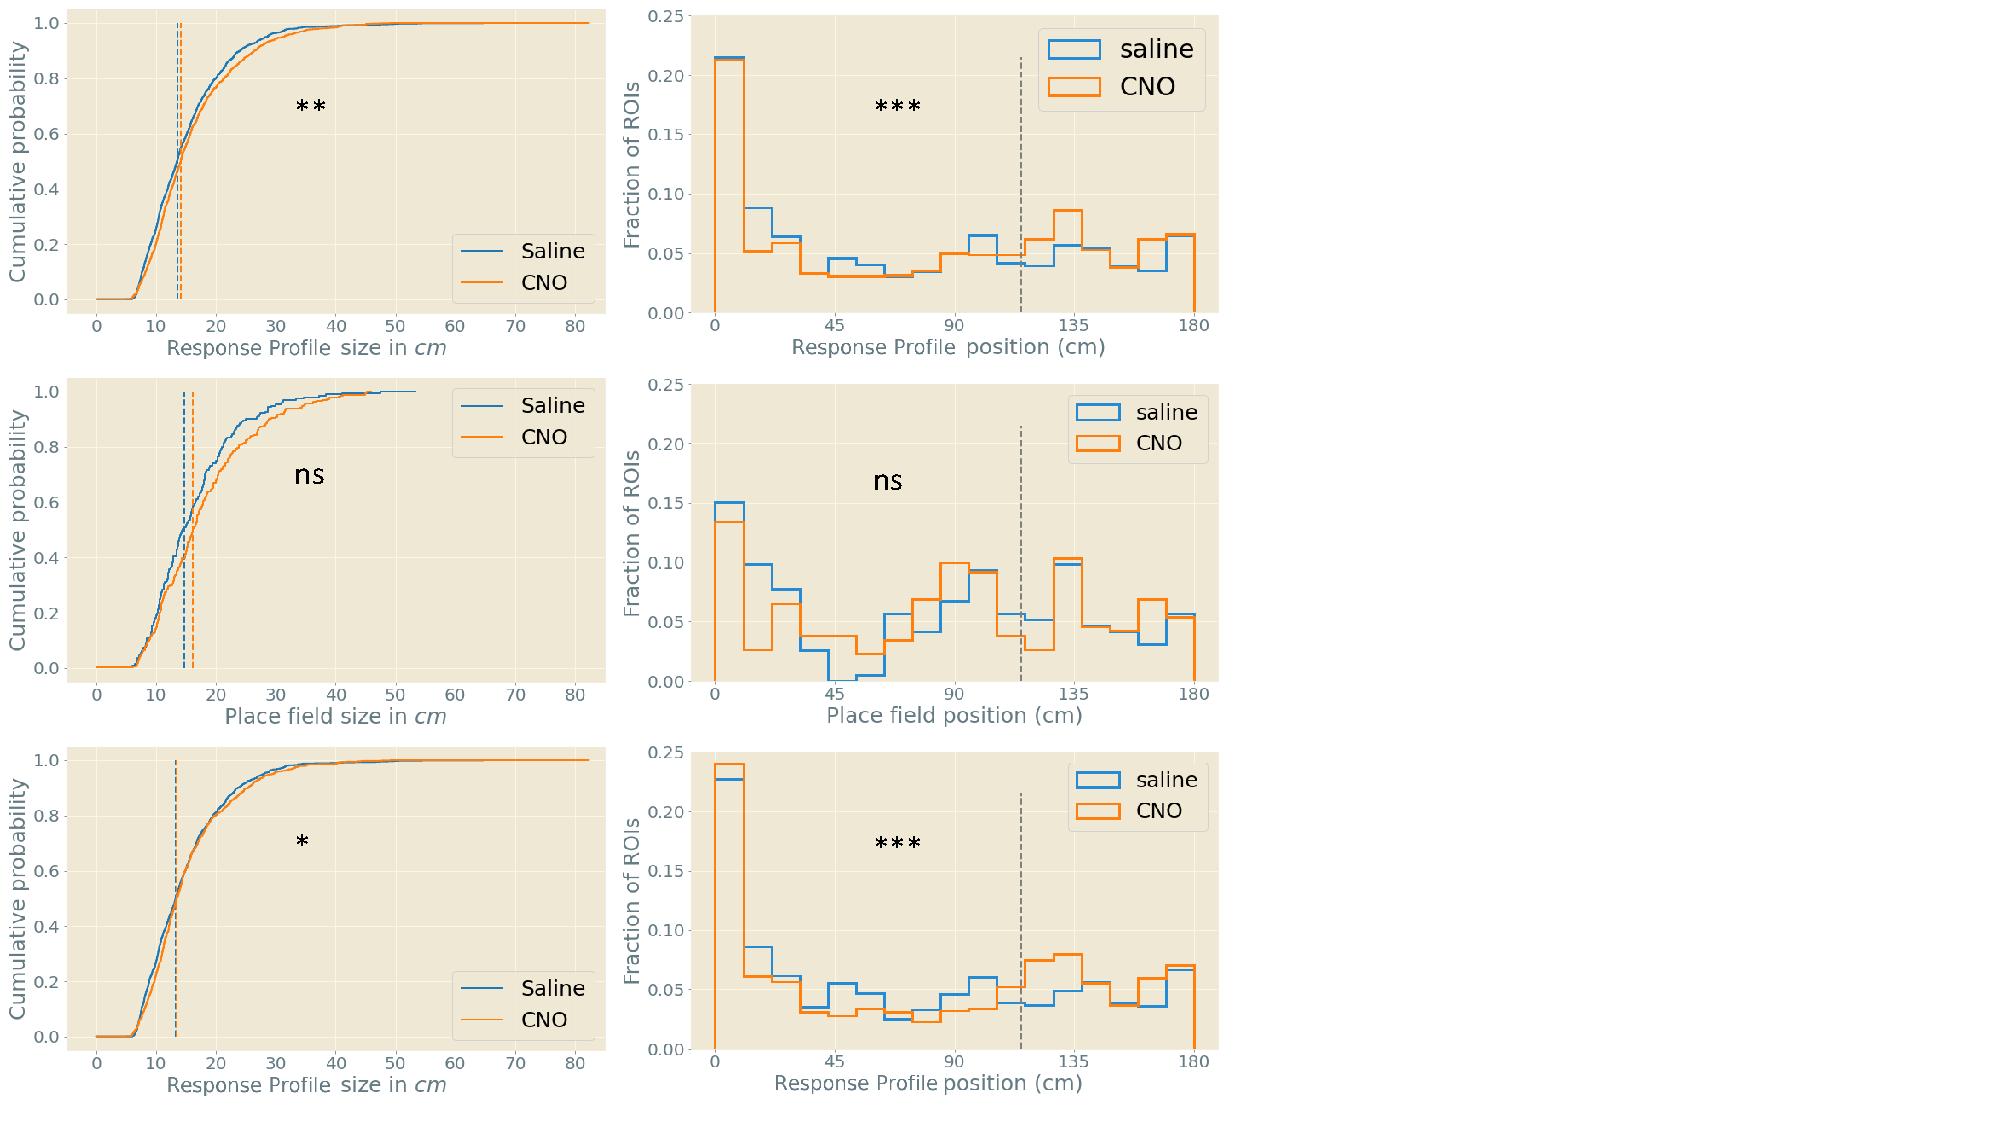
\includegraphics[trim={0 0 360 0},clip,width=\textwidth]{Figures/Chapter4/pf_width_center_2p.pdf}
    \caption[Difference in response profiles and place fields widths and centers after CNO injection and after saline injection]{\textbf{Difference in response profiles and place fields widths and centers after CNO injection and after saline injection.} 
    Distribution of response profiles width (top left panel, kolmogorov-smirnov test $p=0.005$) and centers (top right panel, $p=9 \cdot 10^{-4}$) for all cells detected ($n=1192$ saline, $n=1001$ CNO). 
    Distribution of place fields width (center left panel, $p=0.10$) and centers (center right panel, $p=0.13$) for place cells ($n=193$ saline, $n=261$ CNO).
    Distribution function of response profiles width (bottom left panel, $p=0.03$) and centers (bottom right panel, $p=10^{-4}$) for non-place cells ($n=999$ saline, $n=740$ CNO).}
    \label{fig:chap4:width_center_2p}
\end{figure}
There are, however, two aspects of the data presented that should be considered. 
First, the dataset presented above had large differences in the number of cells detected across FOVs. 
This could in principle introduce biases in the comparisons, with FOVs with a higher number of cells having a larger influence on the result. 
Second, in the dataset described above, different FOVs were imaged under each experimental condition.
Thus, statistical testing of the effect of the treatment (CNO vs. saline injection) was always performed on different sets of neurons, precluding a paired comparison.
To address these limitations, we developed a more accurate protocol to repetitively position the animal under a two-photon microscope, allowing imaging of the same FOV over different experimental sessions (longitudinal recordings) and leading to a larger number of imaged neurons. 
The analysis of this new dataset is presented in the next section.

% =========================================================== %
%          Subsection: Longitudinal recordings                %
% =========================================================== %
\section{Imaging neuronal place cells during pharmacogenetic manipulation of astrocytes in vivo: longitudinal recordings}
\label{chap4:sec:4:longitudinal_recordings}
To study the same population of cells across conditions and across days, we performed longitudinal 2-photon imaging recordings in three sessions: day 0 - saline injection, day 1 - CNO injection, and day 3 - saline injection (see methods \ref{chap3:sec:1:subsec4:long_recordings}).
The new experimental protocol (see methods \ref{chap3:sec:1:subsec4:long_recordings}) allowed us to successfully image the same FOV across sessions, as seen in the representative median projections of the acquired t-series in Figure \ref{fig:chap4:example_longitudinal_FOV}.
Segmentation was performed in the t-series concatenated across days (Figure \ref{fig:chap4:segmentation_long}A) and in individual t-series (Figure \ref{fig:chap4:segmentation_long}B).
To compare segmentations of concatenated vs. individual t-series, we computed the F-1 score, which is defined as: 
\begin{equation*}
    \frac{tp}{tp+\frac{1}{2}(fp+tn)}
\end{equation*}
where $tp$, $fp$ and $tn$ are the true positives, false positives, and true negatives, respectively. The F-1 score ranges between 0 and 1.
In each case, to compute these values, the segmentation of one of the t-series was considered the ground truth, and the other was used for comparison. 
The closer to 1 the F-1 score was, the larger was the overlap between segmentations in different t-series.
In the example shown in fig. \ref{fig:chap4:example_longitudinal_FOV}, the F-1 score varied between 0.75 and 1 for all pairs of recordings (Figure \ref{fig:chap4:segmentation_long}C), meaning that for any pair of t-series, the overlap between segmentation was higher than 75\%.
Identities shared across all 3 recording days (saline, CNO, and saline) and segmentations were considered successfully tracked.
\begin{figure}[h]
    \centering
    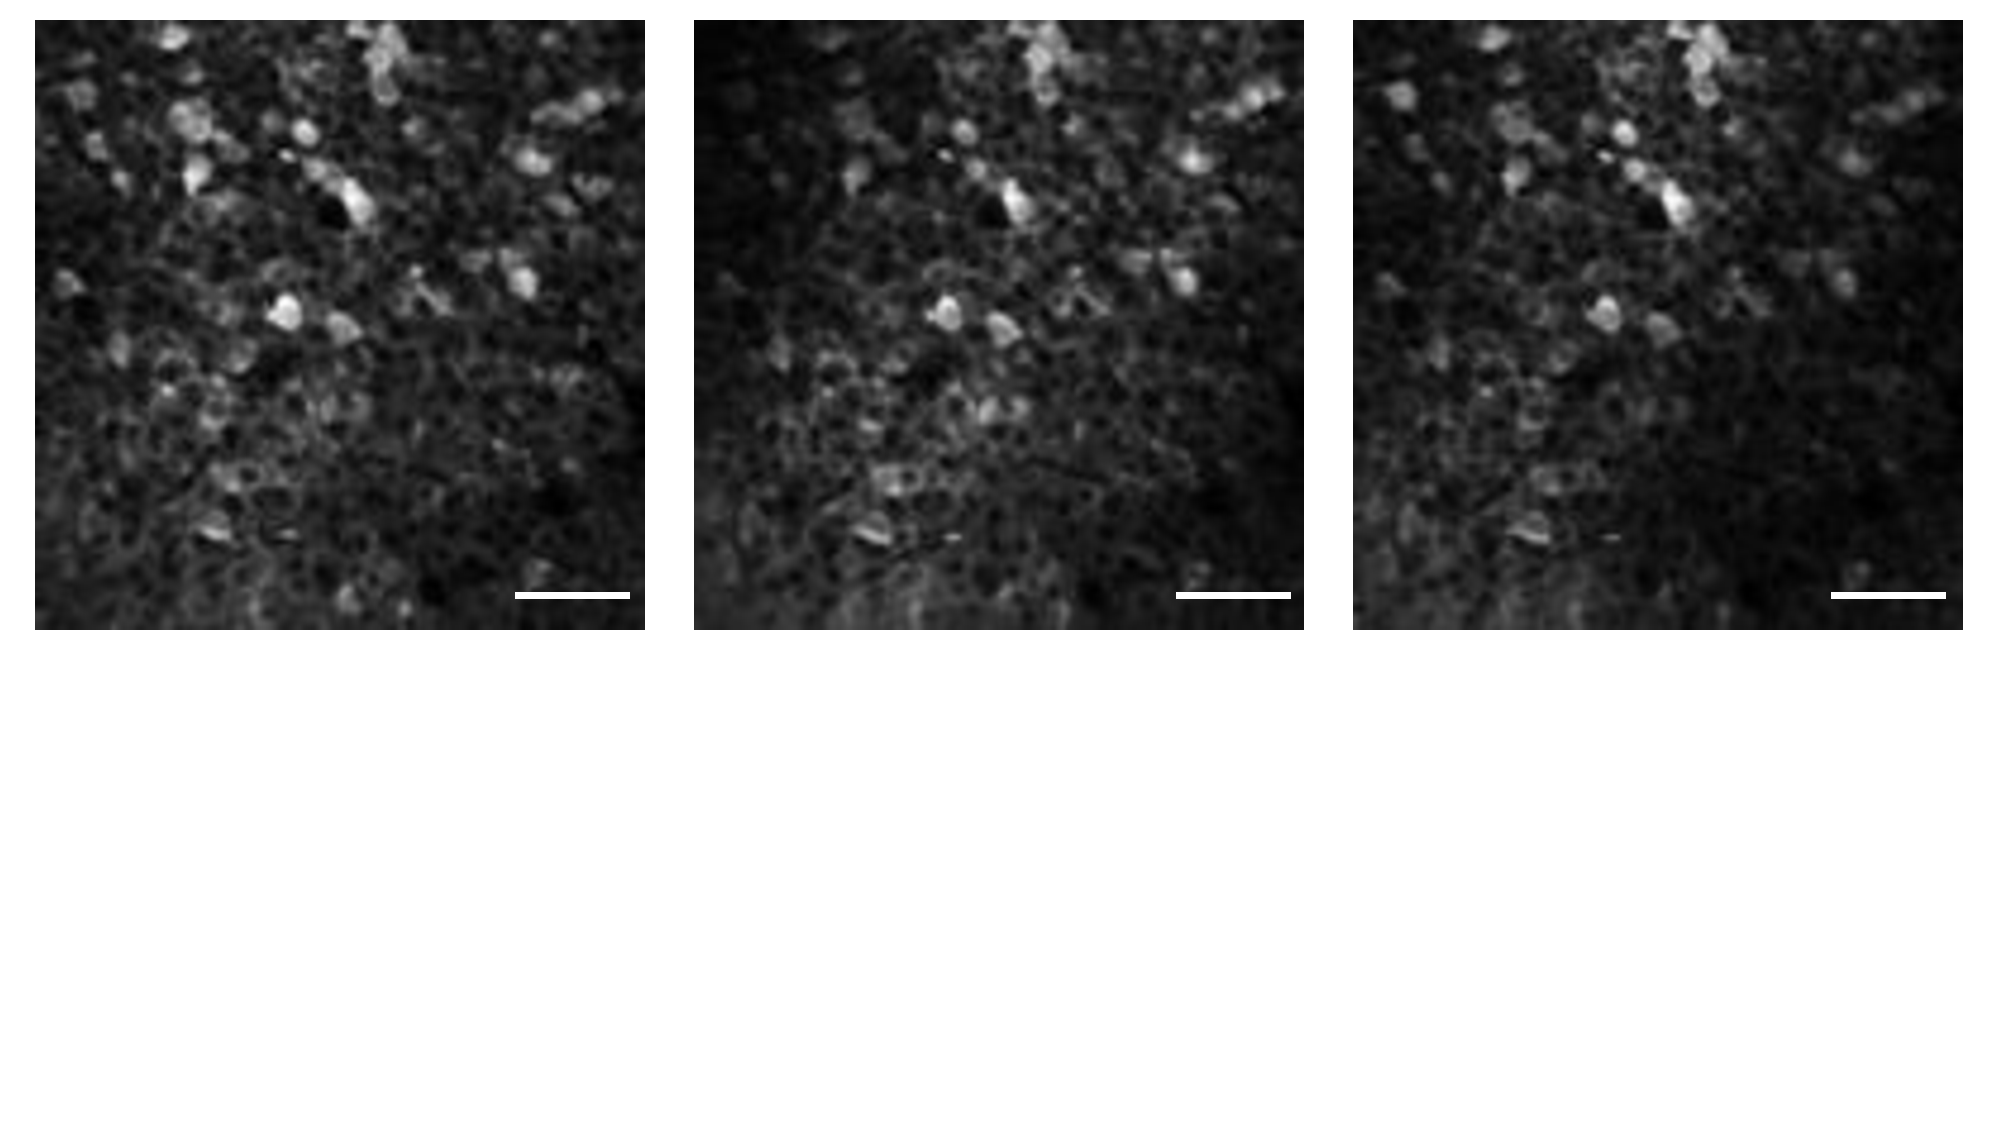
\includegraphics[trim={0 240 0 0},clip,width=\textwidth]{Figures/Chapter4/example_longitudinal_FOV.pdf}
    \caption[Fields of view were successfully tracked and recorded across days]{\textbf{Fields of view were successfully tracked and recorded across days.} 
    From left to right, median projection of first day of saline, CNO and second day of saline injections of a representative FOV (scale $60\ \mu m$}
    \label{fig:chap4:example_longitudinal_FOV}
\end{figure}

We computed the normalized calcium responses of all neurons with significant information content about space, as shown in Figure \ref{fig:chap4:snake_plot_2p}, for each of the 3 days of recordings (Figure \ref{fig:chap4:snake_plots_long}). 
Identities were ordered according to the position of the center of the response field in increasing order.
The first day of saline injection recordings is shown in the left panel, CNO injection recordings are shown in the middle panel, and the second day of saline recordings is shown in the right panel (488, 476 and 472 informative  ROIs out of 1740, 1708 and 1758 total, respectively).
As in the nonlongitudinal recordings, in every condition, PF spans the whole trace, allowing for the complete mapping of space regardless of treatment.
Recordings from 3 animals were analyzed.
\begin{figure}
    \centering
    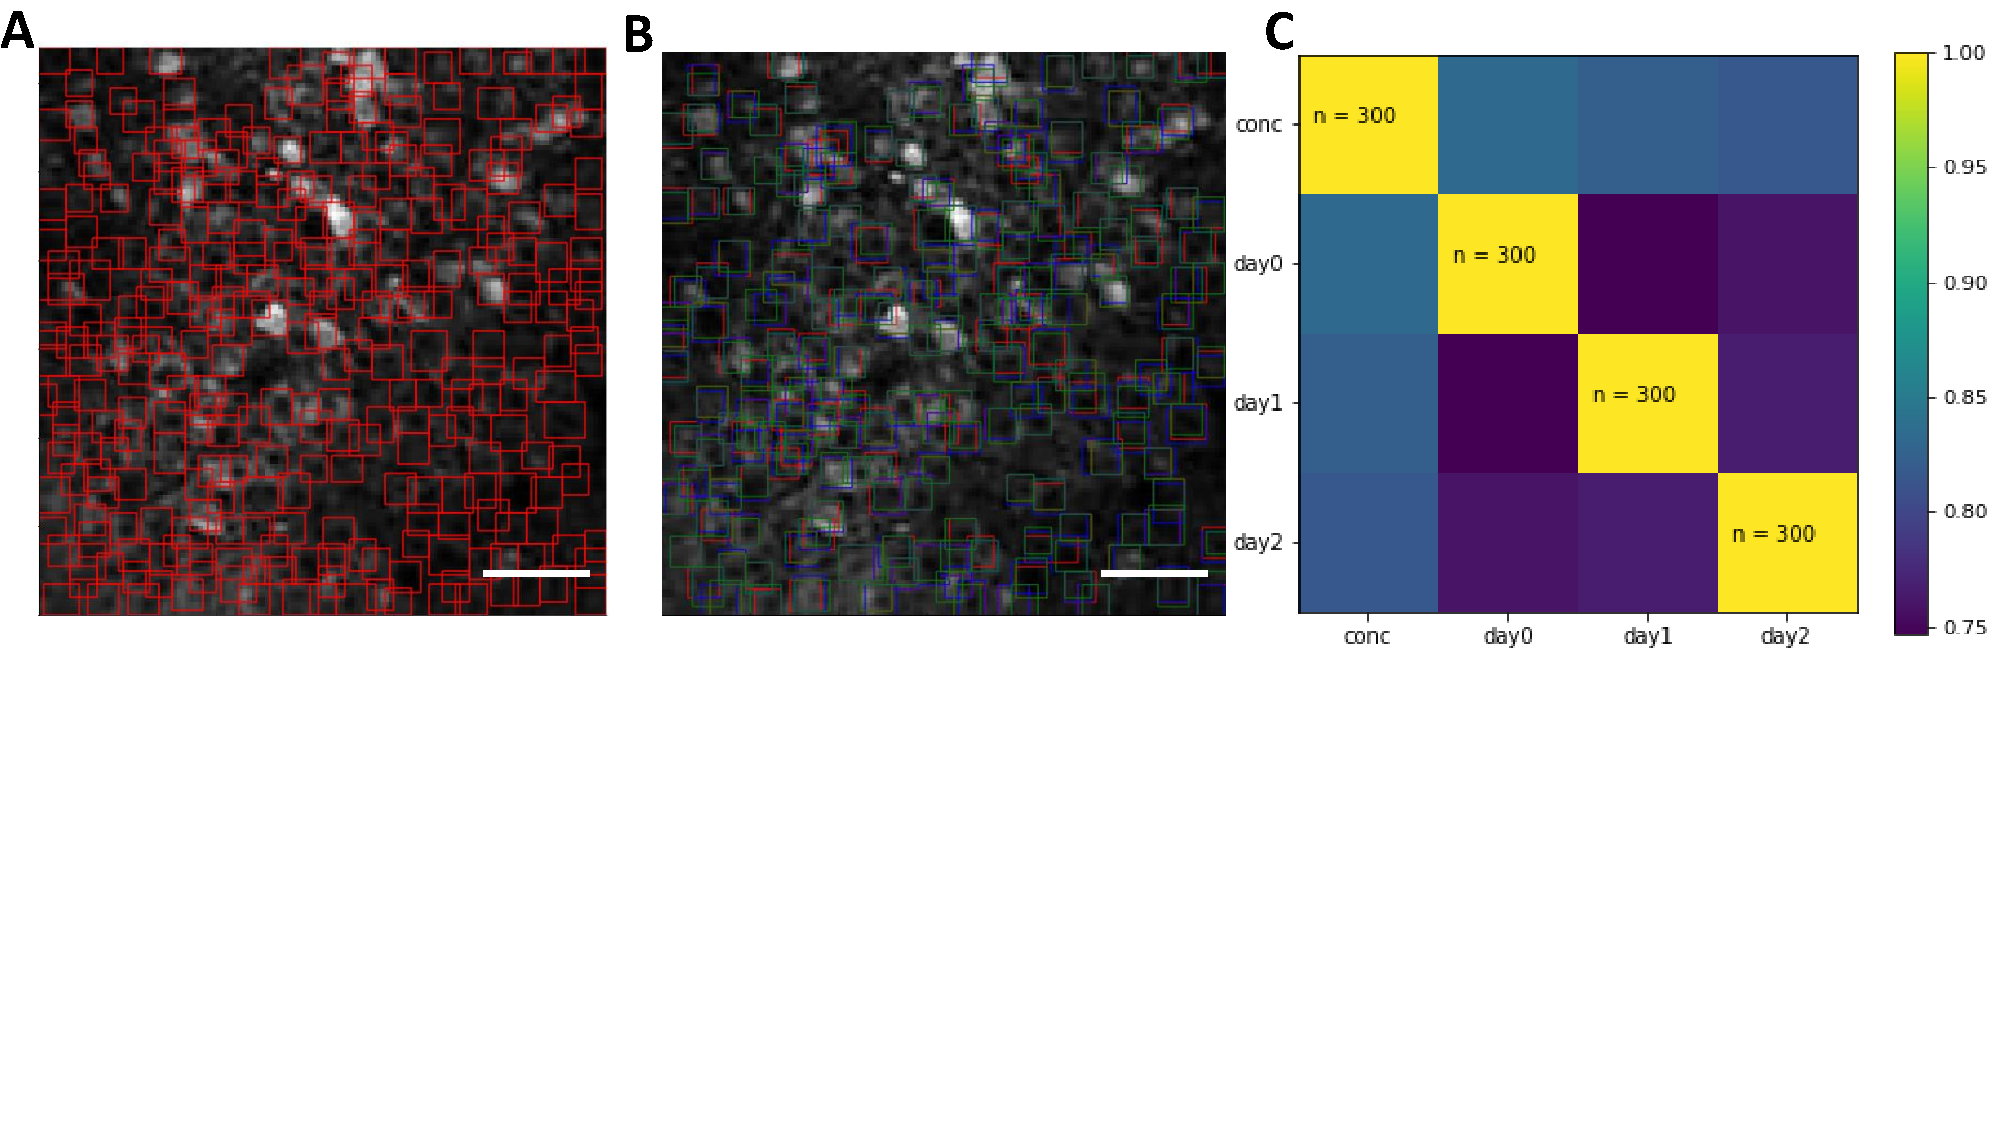
\includegraphics[trim={0 230 0 0},clip,width=\textwidth]{Figures/Chapter4/segmentation_long.pdf}
    \caption[Segmentation and ROI tracking in longitudinal recordings]{\textbf{Segmentation and ROI tracking in longitudinal recordings.} 
    A) Segmented boxes (red) performed on the concatenated recording median projection of a two-photon t-series (scale $60\ \mu m$). 
    B) Segmentation from different recording days are shown superimposed. Identities successfully tracked across days are shown in red, green and blue for each day respectively (190 tracked identities out of 300 total, scale as in A). 
    C) F-1 matrix for detections performed in the concatenated t-series and the 3 different days.}
    \label{fig:chap4:segmentation_long}
\end{figure}

To study how alterations in astrocytic calcium activity influenced spatial mapping in the same population of neurons, we first compared the distributions of MI values after saline (first and second day) or CNO injection for each animal with the non-longitudinal recordings (section \ref{chap4:sec:3:linear_track}).
Boxplots and statistical tests are reported in each of the 6 panels of Figure \ref{fig:chap4:MI_C_all_cells_longitudinal}.
\begin{SCfigure}[][h]
    \centering
    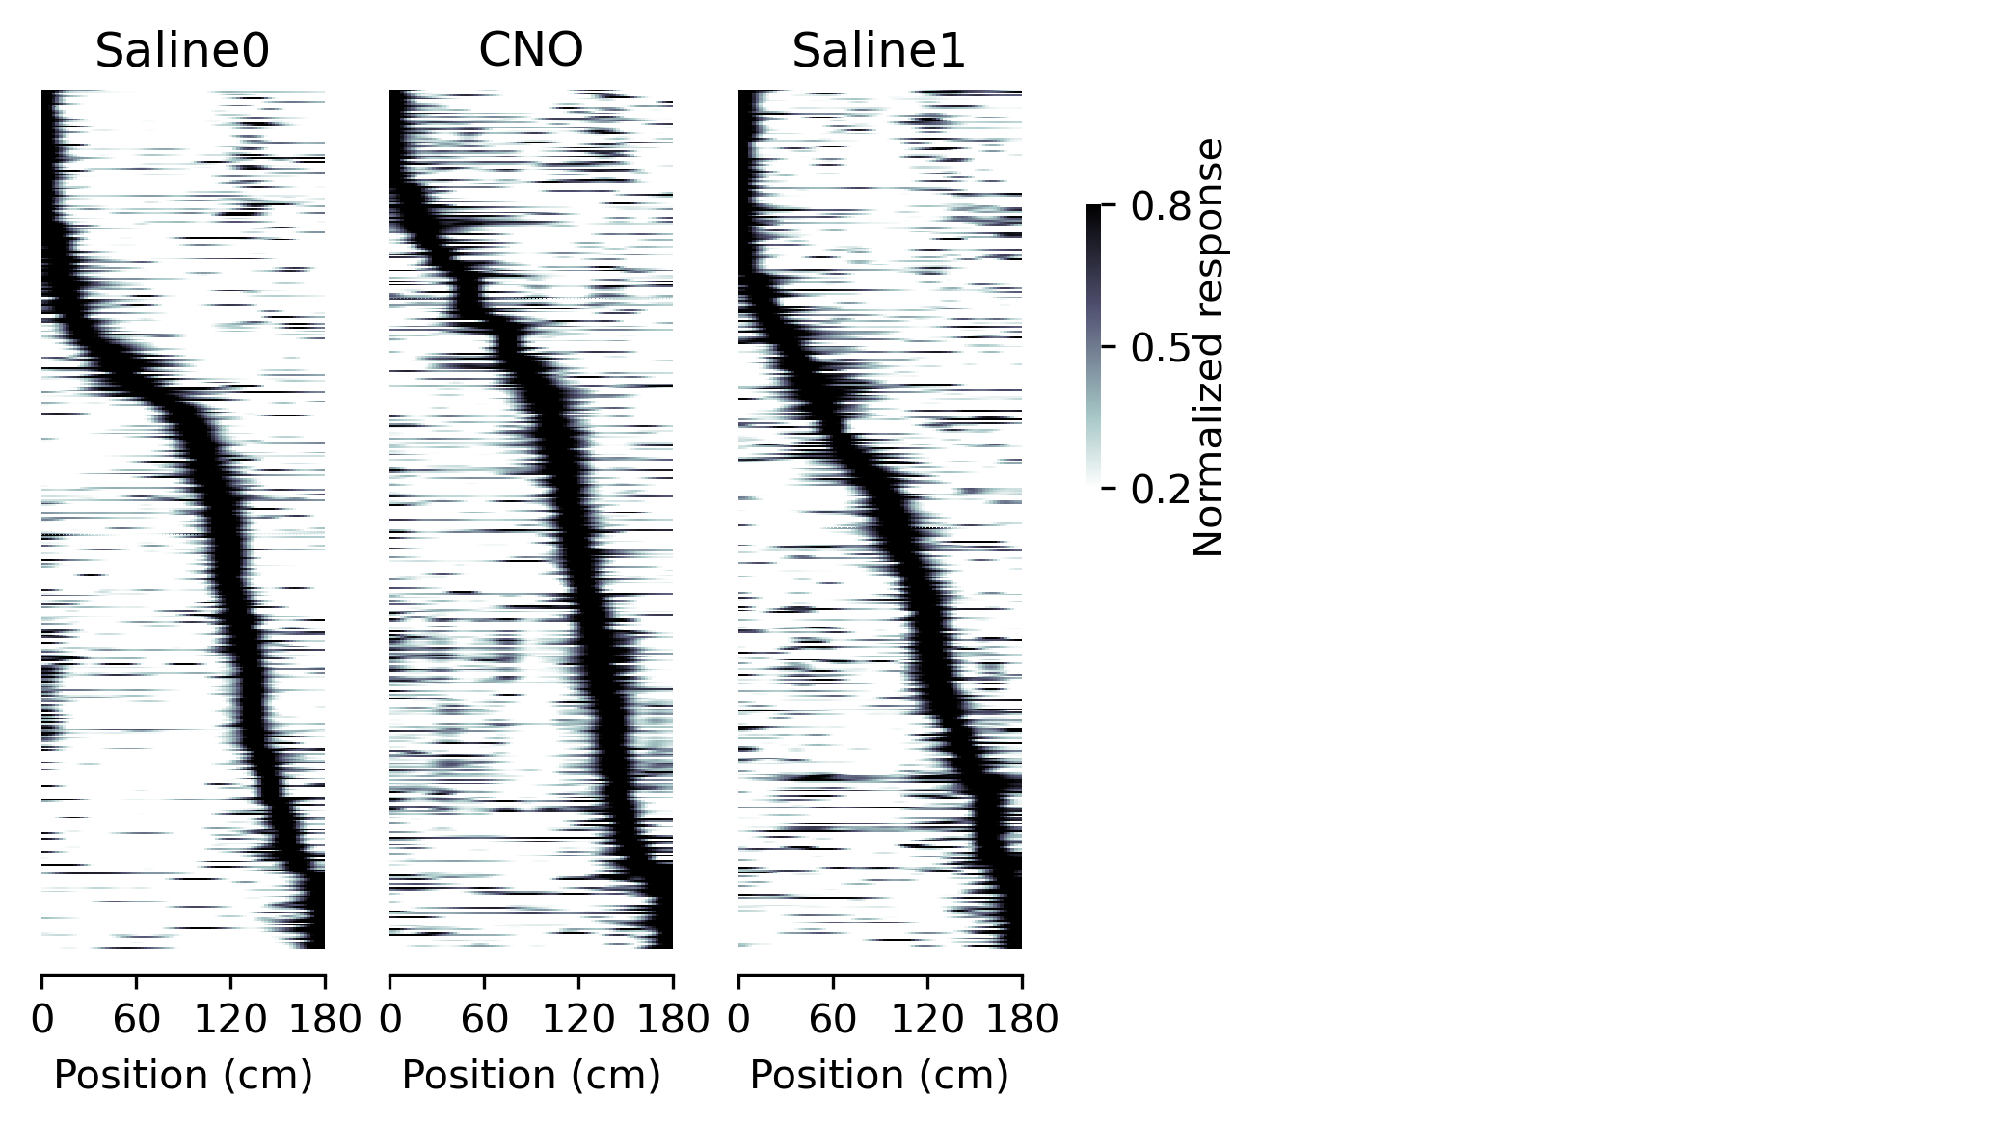
\includegraphics[trim={0 0 450 0},clip,width=0.5\textwidth]{Figures/Chapter4/snake_plots_long.pdf}
    \caption[Normalized calcium responses as a function of position for neurons that contain significant amount of spatial information]{\textbf{Normalized calcium responses as a function of position for neurons that contain significant amount of spatial information.} 
    Left panel, responses from recordings in which the animal was injected with saline solution (n = 488 informative ROIs out of 1740 total ROIs, 6 imaging sessions from 6 FOVs). 
    Center panel, responses from recordings in which the animal was injected with CNO solution (n = 476 informative ROIs out of 1708 total ROIs, 6 imaging sessions from 6 FOVs). 
    Right panel, responses from recordings in which the animal was injected with saline solution after the CNO day (n = 472 informative ROIs out of 1758 total ROIs, 6 imaging sessions from 6 FOVs). 
    Responses are ordered according to the position of the center of the response field (from minimum to maximum).}
    \label{fig:chap4:snake_plots_long}
\end{SCfigure}
Both place cells and nonspatial encoding cells were pooled together; thus, the distributions were centered close to zero and heavy tailed towards positive values.
Distributions of MI across conditions showed heterogeneous behavior across animals, and in contrast to observations for nonlongitudinal recordings, the difference in the averages was not significantly different for any of the comparisons between conditions (\ref{fig:chap4:MI_C_all_cells_longitudinal} right-most panel, Wilcoxon paired test with Bonferroni correction; saline 0 vs. CNO, $p=0.91$; saline 0 vs. saline 1, $p=0.91$; CNO vs. saline 1, $p=0.34$).

To account for FOV variability and asymmetries in the number of elements per condition per animal, we again used an LMEM with treatment as a fixed effect and FOV as a random effect with either a random intercept (LME1) or a random intercept and a random slope (LME2).
First, we fitted an LME2 model, considering only treatment as the fixed effect.
The fitted slope of the LME2 model was small, at $5\cdot 10^{-4}$, and positive, which implies a small increase in the information content on saline days.
In contrast to observations for nonlongitudinal recordings, the effect of treatment was found to be statistically nonsignificant (Type II Wald chi-square tests, $p=0.87$).
We then examined the effect of CNO injection when considering only place cell information content. We fitted an LME1 model with similar results-the fitted slope was 0.001, and the effect was nonsignificant ($p=0.87$).
\begin{figure}[h]
    \centering
    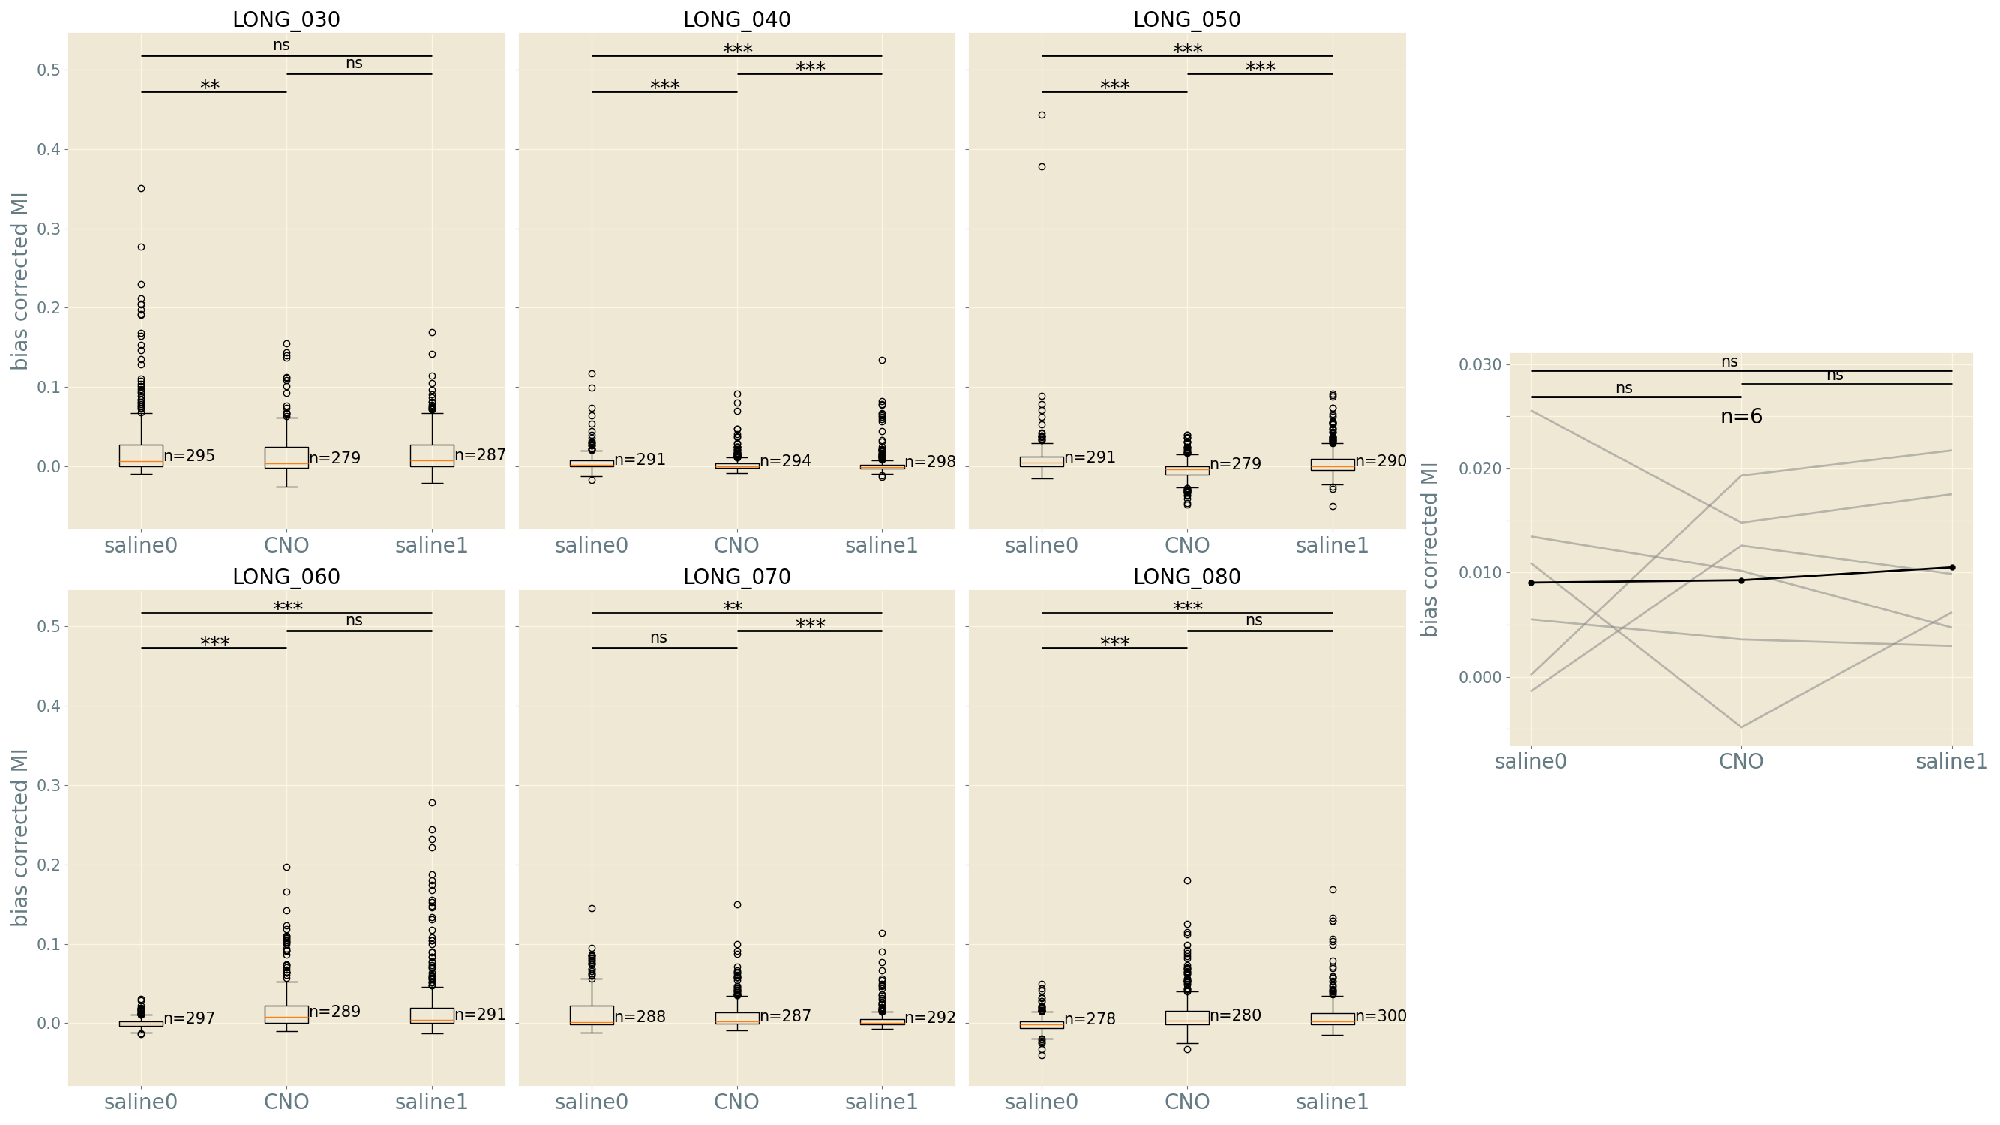
\includegraphics[width=\textwidth]{Figures/Chapter4/MI_C_all_cells_longitudinal.pdf}
    \caption[Bias corrected MI distributions under the different experimental conditions]{\textbf{Bias corrected MI distributions under the different experimental conditions.} Each panel represents a different FOV, with the box plots of MI distributions for first saline injection day, CNO injection day, and second saline injection day. Panels in the same column correspond to the same animal. Right-most panel shows the difference between MI values averages for each FOV (gray lines) and the overall average (black line), with no significant difference between different days (Wilcoxon paired test with Bonferroni correction, saline 0 vs CNO $p=0.91$; saline 0 vs saline 1 $p=0.91$; CNO vs saline 1 $p=0.34$)}
    \label{fig:chap4:MI_C_all_cells_longitudinal}
\end{figure}

In doing this analysis, we pooled together two different days of saline injection, with one taking place before and one after the CNO injection day. 
To better compare the results of the analysis of this dataset with those of the nonlongitudinal recording (wherein only one saline condition was available), we limited the analysis to the first day of saline injection and the following CNO injection day.
We fitted an LME2 model for all cells and found that the effect of the treatment was not significant ($p=0.96$) and that the slope was negative, at $-2\cdot 10^-4$.
We then fitted an LME1 model, taking into consideration only place cells from the first two days and obtained a fitted slope of -0.001 (10\% decrease on saline day, $p=0.57$).
Finally, we fitted the LME2 model to compare the two saline days, and again, we found no statistically significant difference ($p=0.74$).  

We then compared the center and width of the response profiles and/or place fields for the first day of the saline injection and CNO injection experiments (Figure \ref{fig:chap4:pf_width_center_long}).
When considering all cells, the response profile width was not significantly different after CNO injection (Figure \ref{fig:chap4:pf_width_center_long} top left panel, Kolmogorov-Smirnov test, $p=0.62$).
The distributions of response profile centers were significantly different (Figure \ref{fig:chap4:pf_width_center_long} top right panel, $p=0.009$).
When considering the subset formed by only place cells and observing place field widths and centers (Figure \ref{fig:chap4:pf_width_center_long} bottom left and right panels, respectively), we observed a statistically significant increase in PF width ($p=8.8 \cdot 10^{-6}$) and a significant difference between PF center distributions ($p=0.001$).
\begin{figure}
    \centering
    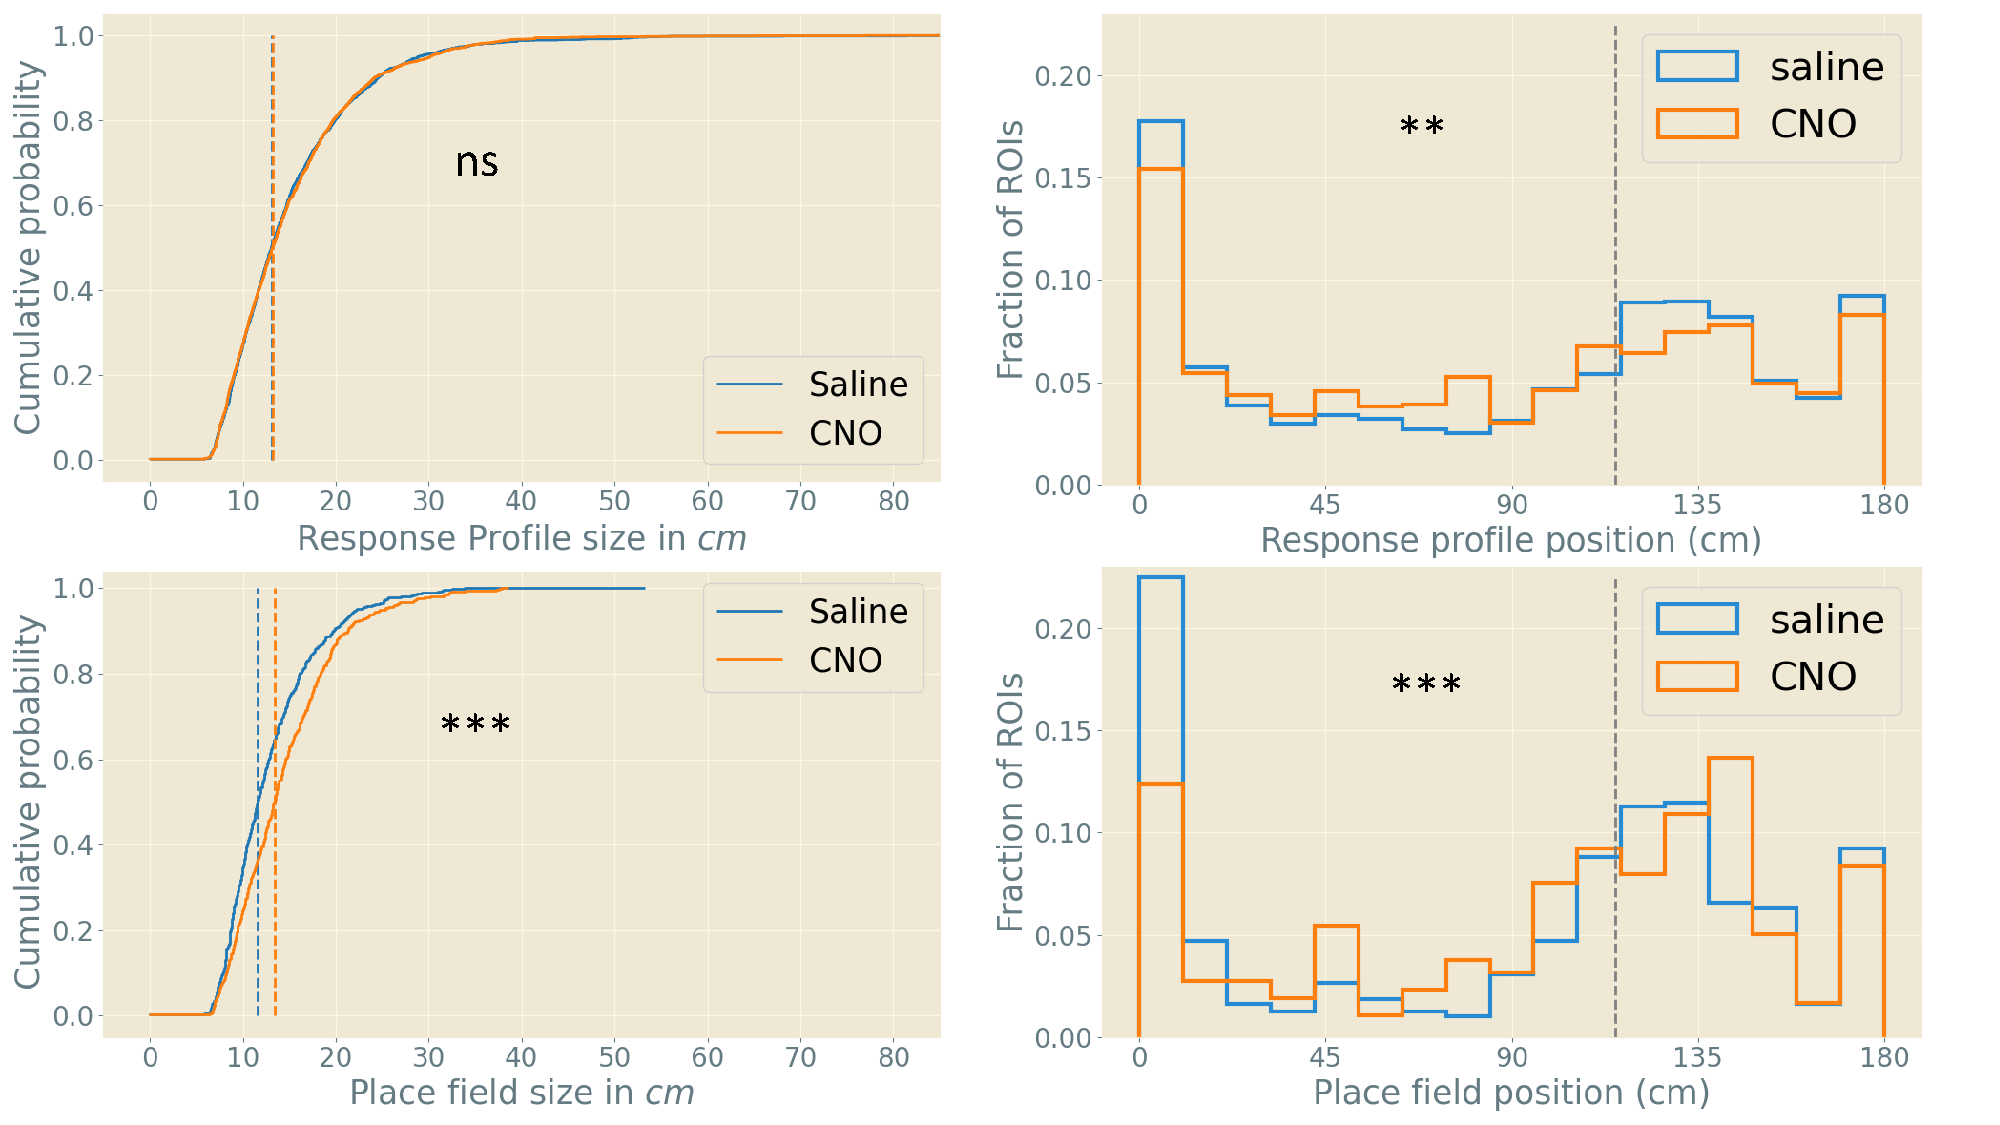
\includegraphics[width=\textwidth]{Figures/Chapter4/pf_width_center_long.pdf}
    \caption[Response profiles, place field widths, and place field centers in CNO and saline for longitudinal recordings]{\textbf{Response profiles, place field widths, and place field centers in CNO and saline for longitudinal recordings.} 
    Distribution of response profiles width (top left panel, kolmogorov-smirnov test $p=0.62$) and centers (top right panel, $p=0.009$) for all cells detected.
    Distribution of place fields width (bottom left panel, $p=8.8 \cdot 10^{-6}$) and centers (bottom right panel, $p=0.001$) for place cells.}
    \label{fig:chap4:pf_width_center_long}
\end{figure}

We then analyzed the effect of CNO injection \textbf{on the same cells}. 
For this, we tracked cell identities belonging to the same FOV across days (see methods \ref{chap3:sec:5:long_tracking}).
We first compared the MI values for each cell across days (Figure \ref{fig:chap4:MI_C_tracked_cells_longitudinal}).
The differences and results were heterogeneous and did not show statistically significant differences across days on average (Figure \ref{fig:chap4:MI_C_tracked_cells_longitudinal} right-most panel, Wilcoxon paired test with Bonferroni correction, saline 0 vs. CNO, $p=0.91$; saline 0 vs. saline 1, $p=0.91$; CNO vs. saline 1, $p=0.34$).
Note that these values are a subset of the data shown in figure \ref{fig:chap4:MI_C_all_cells_longitudinal}, but here, each line represents one cell that has been tracked across all 3 days. 
\begin{figure}
    \centering
    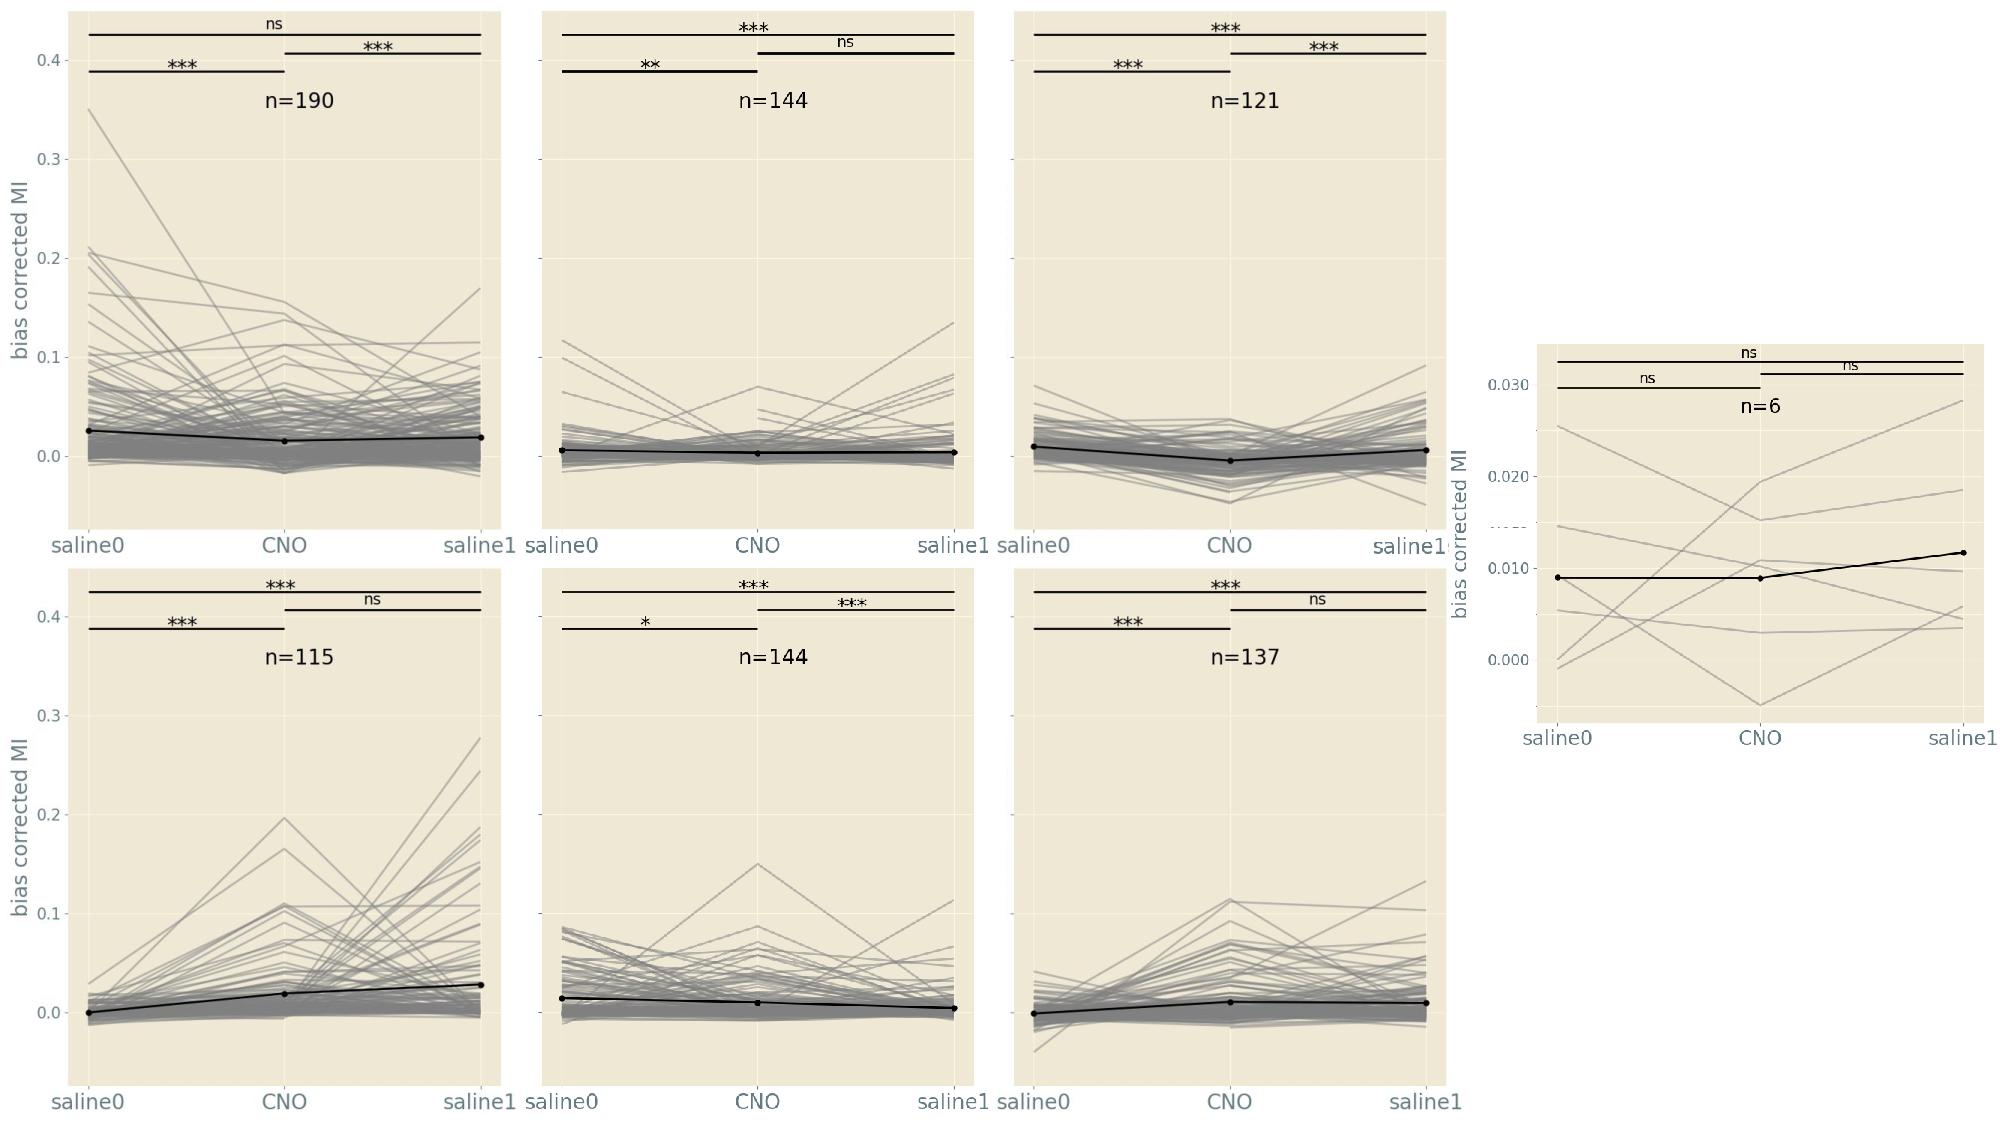
\includegraphics[width=\textwidth]{Figures/Chapter4/MI_C_tracked_cells_longitudinal.pdf}
    \caption[Bias corrected MI values for tracked cells across days]{\textbf{Bias corrected MI values for tracked cells across days.} 
    Each gray line corresponds to a tracked ROI and black lines to averages. 
    Missing points (interrupted lines) correspond to cells that were silent in one of the days (paired Wilcoxon tests with Bonferroni correction where performed in each case). 
    Information could not be computed in sessions in which neurons did not show activity. 
    Right-most panel shows the difference between MI values averages for each FOV (gray lines) and the overall average (black line), with no significant difference between different days (Wilcoxon paired test with Bonferroni correction, saline 0 vs CNO $p=0.91$; saline 0 vs saline 1 $p=0.91$; CNO vs saline 1 $p=0.34$) }
    \label{fig:chap4:MI_C_tracked_cells_longitudinal}
\end{figure}

Finally, we studied cell-wise variation in the place field and response profile widths and centers.
We computed the difference between CNO and saline (first application) response profile centers for all tracked cells in all FOVs. 
The histogram of the differences showed an approximately symmetric distribution with respect to zero (Figure \ref{fig:chap4:width_center_tracked_cells_longitudinal} top right panel), with a higher number of cells in the two central bins, meaning that a high percentage of cells tended to maintain their response profile centers. 
We asked whether variations in response centers could be related to differences in information content. 
In the top lef panel of Figure \ref{fig:chap4:width_center_tracked_cells_longitudinal}, we can see the distributions of tracked cells in the plain defined by the centers of the response profile in each day.
Each circle represents a tracked cell, and its color represents the difference in the MI value (CNO minus saline 0).
No clear asymmetry in the distribution of cells in the plane or relationship with the change in information content was observed, besides the higher number of dots on the diagonal (as expected from the histogram), regardless of the variation in the MI content.
Similarly, we computed the differences in the response profile width, with the vast majority of cells having a variation of less than $20 cm$ (Figure \ref{fig:chap4:width_center_tracked_cells_longitudinal} bottom right panel).
This was further confirmed by the distribution in the plain defined by the width on different days (Figure \ref{fig:chap4:width_center_tracked_cells_longitudinal} bottom left panel), which also had no clear relationship with the difference in MI values. 
\begin{figure}
    \centering
    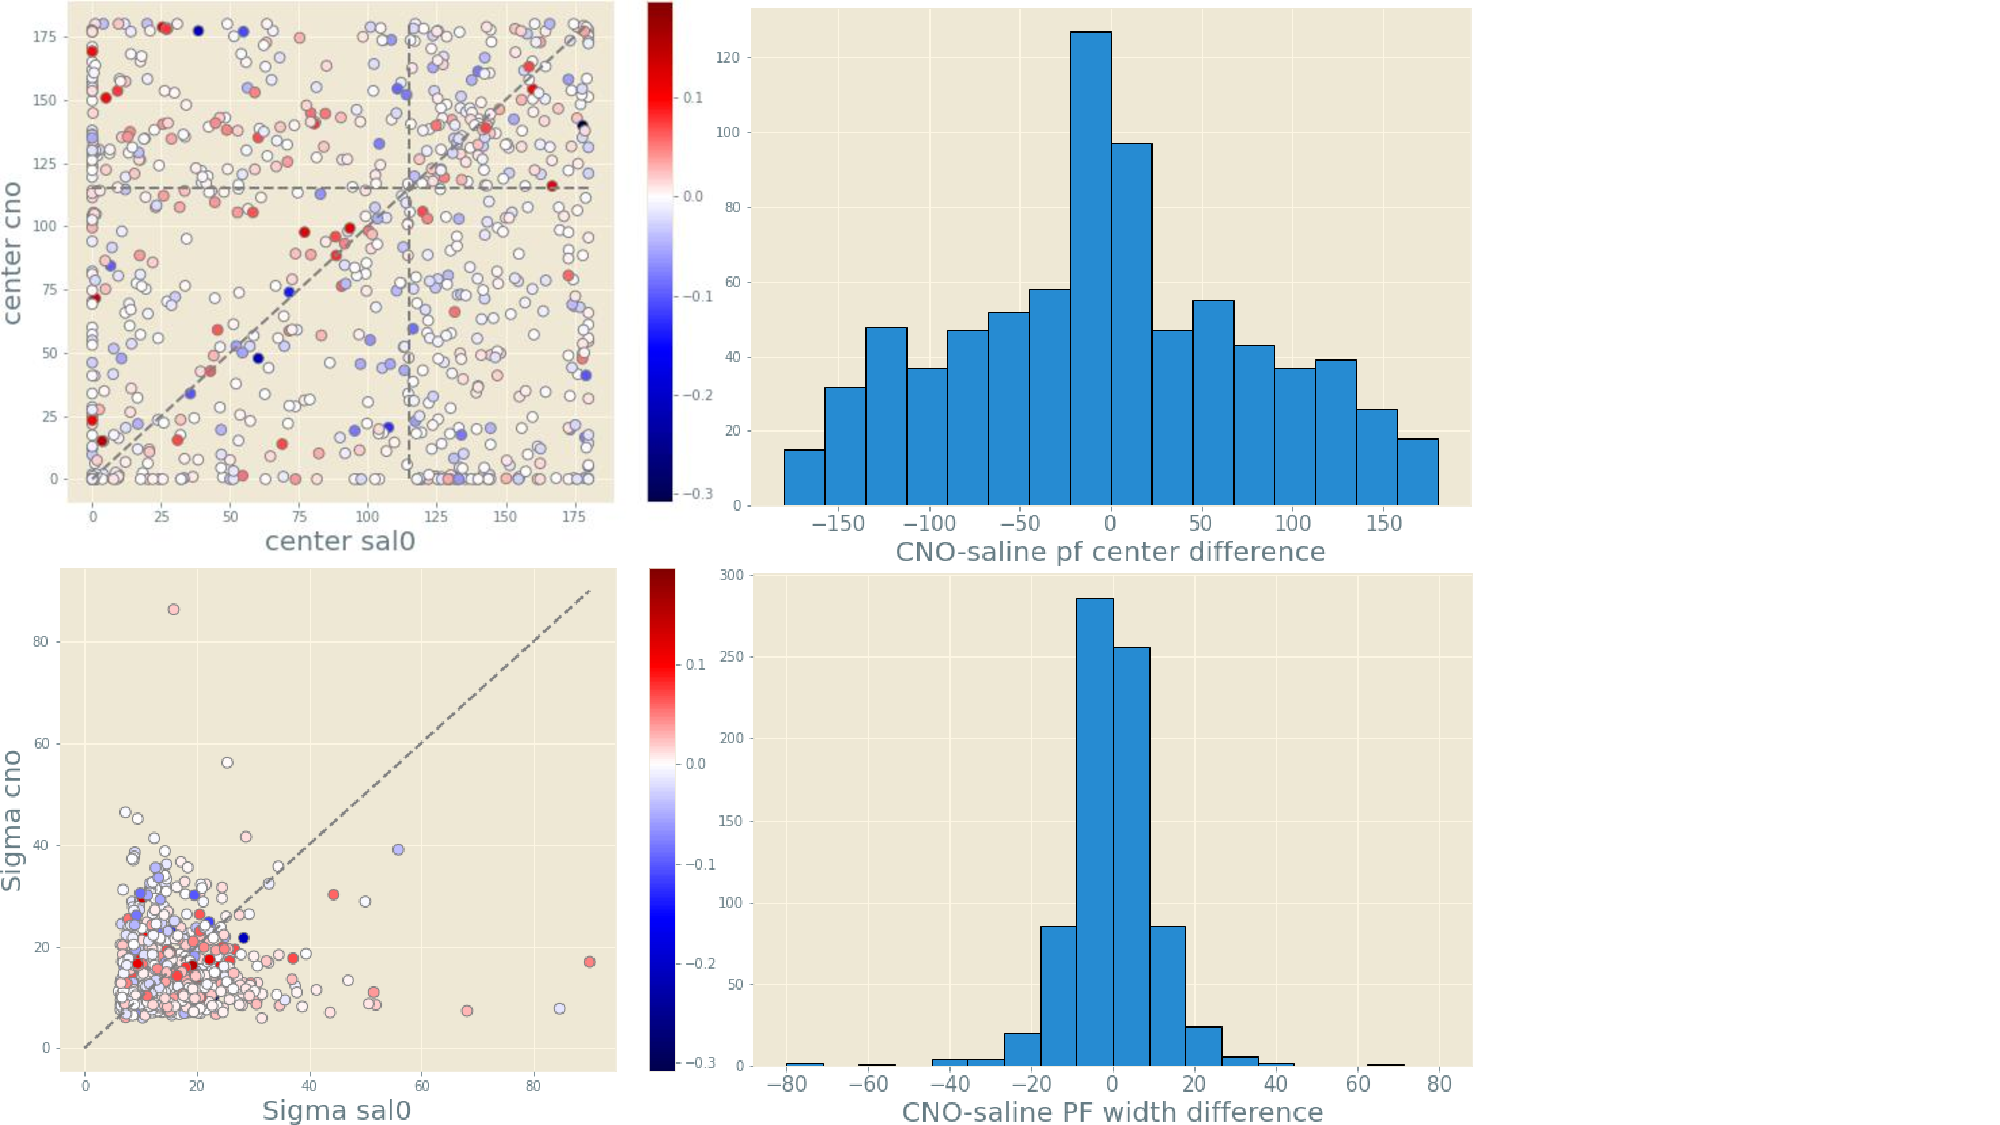
\includegraphics[trim={0 0 250 0},clip,width=\textwidth]{Figures/Chapter4/width_center_tracked_cells_longitudinal.pdf}
    \caption[Place field width and center difference for tracked cells between first day of saline injection vs CNO injection]{\textbf{Place field width and center difference for tracked cells between first day of saline injection vs CNO injection.} Top left panel shows position of PF centers in CNO day vs Saline 0 day, each dot is a cell and the color of the dot represents the difference in MI values between CNO minus Saline 0, dotted gray lines are the diagonal (representing equal centers position) and the reward location for each day. Top right panel, histogram of the difference between CNO minus Saline 0 days PF centers. Bottom panels as top panels for width of place fields.}
    \label{fig:chap4:width_center_tracked_cells_longitudinal}
\end{figure}

Taken together, the analysis of the longitudinal recordings showed that CNO application did not have major effects on the content of information or on the features of neuronal place cells, in contrast to the results of the nonlongitudinal recordings.
We discuss these contrasting results in the following section.